\documentclass[11pt,a4paper]{ctexart}

\usepackage[a4paper,margin=0.95in]{geometry}
\usepackage{booktabs}
\usepackage{tabularx}
\usepackage{graphicx}
\usepackage{subcaption}
\usepackage{float}
\usepackage{enumitem}
\usepackage[hidelinks]{hyperref}
\usepackage{xcolor}
\usepackage[numbers,sort&compress]{natbib}

\setlist[itemize]{leftmargin=*,itemsep=2pt,topsep=2pt}
\setlist[enumerate]{leftmargin=*,itemsep=2pt,topsep=2pt}

% 图表标题样式：比正文小一号，标签加粗，与正文形成层次区分
\captionsetup{
  font=small,
  labelfont=bf,
  skip=6pt
}

\newcommand{\dataset}{Nemotron-Personas-France}
\newcommand{\ifop}{IFOP}
\newcommand{\stance}{\textit{stance}}
\newcommand{\score}{\textit{support\_score}}

\title{\textbf{大语言模型生成社会调查数据的统计真实性评估}\\
\large 基于法国人物画像与退休改革议题的数据科学课程项目报告}
\author{胡浩然 \quad 何俊豪 \quad 仇炎 \quad 魏兰馨\\
南京大学 信息管理学院}
\date{}

\begin{document}
\maketitle

\begin{abstract}
本项目围绕“如何评估大语言模型生成社会调查数据的统计真实性”展开。我们从 Hugging Face 上的 \dataset{} 合成人物画像数据集出发，将其中的法国居民画像视为“虚拟受访者”，并以法国退休改革为案例，构建了一套从人物画像抽样、Prompt Context 设计、LLM 调用、JSON 解析、质量审计到主数据集分析的完整流程。项目使用 \ifop{} 真实民调作为宏观参照，首先通过 Prompt $\times$ Sampling 交叉实验筛选主数据生成方案，最终形成 9,960 条有效模拟调查记录，并进一步开展探索性分析、特征工程、机器学习建模、标签稳定性检验和少数类优化实验。结果表明，LLM 模拟数据能够呈现一定的群体层面结构，例如年龄与支持度之间的方向性关系；但在个体层面，模型解释力有限，最佳回归模型的测试集 $R^2$ 约为 0.206，分类模型也难以稳定识别少数类 \textit{oppose}。进一步诊断发现，这种限制并不只是算法问题，还与人物画像缺少近端政治变量、标签重复生成不稳定、少数类语义边界模糊等因素有关。因此，本项目的结论不是“LLM 可以替代真实民调”，而是：LLM 生成社会调查数据可以作为一种探索性数据资源，但必须结合真实基准、抽样审计、稳定性检验和误差诊断来评估其统计真实性。
\end{abstract}

\begin{center}
\textbf{关键词：} 大语言模型；计算社会科学；合成调查；统计真实性；人物画像；民意模拟
\end{center}

\section{引言：从人物画像到生成式社会调查}
计算社会科学强调利用大规模数据和计算方法研究社会现象 \cite{lazer2009computational}。随着大语言模型的发展，一个新的问题逐渐出现：模型是否不仅可以分析社会数据，还可以基于人物画像生成类似“受访者”的态度回答？已有研究提出了“silicon samples”等概念，认为在一定条件下，语言模型可能复现部分群体层面的调查分布 \cite{argyle2023out,aher2023using}。但另一方面，机器行为研究也提醒我们，不能把模型输出直接等同于真实人类行为，而应当把它作为一种需要被经验检验的行为对象 \cite{rahwan2019machine}。

从研究前景看，LLM 模拟社会调查的吸引力在于它可能降低试探性调查成本、快速生成假设、补充少数群体或难接触群体的态度线索，并为政策情景推演提供可重复的实验环境。近年的相关研究已经开始将 LLM 作为“合成受访者”或“社会行为模拟器”使用，用真实调查数据检验其回答分布是否与人类样本接近 \cite{argyle2023out,geng2024chameleons}。但这个领域的核心争议同样清楚：LLM 可能复制训练语料中的社会偏见，也可能把复杂人群压缩成过于平均、过于稳定的回答模式；不同 prompt、选项顺序、persona 信息量和模型版本都会显著改变结果。因此，当前更稳妥的研究立场不是把 LLM 当作真实民调替代品，而是把它当作一种“可诊断的生成式社会数据来源”，重点评估其统计真实性、稳健性和失真边界。

本项目正是在这一背景下展开的。我们的研究并不是先确定一个固定问题，再寻找合适数据；相反，它是一条比较典型的数据驱动路径。最开始，我们发现了 \dataset{} 数据集。该数据集包含约 100 万个合成法国居民画像，每个画像不仅有人口统计信息，还包含职业、生活方式、兴趣、文化背景等多维文本描述。看到这批数据后，我们首先思考的是：如此丰富的人物画像是否可以支持一种“虚拟社会调查”？

因此，我们提出了项目设想：将每个 persona 视为一个虚拟受访者，让大语言模型基于其个人画像，对法国退休改革这一具体公共政策问题作出态度判断。进一步地，我们希望回答三个问题：

\begin{enumerate}
  \item LLM 生成的模拟民调，在宏观分布上能否接近真实社会调查？
  \item 人物画像中的哪些特征能够解释模拟态度？机器学习模型能学到多少？
  \item 如果模型效果有限，问题主要来自算法、特征，还是模拟标签本身？
\end{enumerate}

这三个问题共同构成了本项目的主线。我们并不试图证明 LLM 可以替代真实民调，而是希望通过完整的数据科学流程，评估其生成社会调查数据的统计真实性：它是否能在总体分布、群体差异、文本解释、标签稳定性和下游可预测性上表现出可被验证的社会结构信号。

同时，本文按照课程项目报告而非正式投稿论文的方式组织。我们在文献脉络中说明项目动机，在系统设计中说明数据如何产生，在实验部分呈现模型表现和诊断结果，最后回到数据设计反思。

\subsection{理论支撑：计算社会科学、机器行为与 LLM 模拟调查}
 Lazer 等人提出的计算社会科学框架，为本项目提供了基本问题意识：社会态度可以通过大规模数据、计算模型和统计分析进行研究 \cite{lazer2009computational}。Rahwan 等人进一步提出“机器行为”研究，强调应当像研究人类或组织行为一样，经验性地研究算法系统的输出规律 \cite{rahwan2019machine}。在本项目中，大语言模型既是生成数据的工具，也是被观察的对象。我们关心的不只是它能否生成回答，也关心它在不同人物画像、不同立场和不同标签上的系统性表现。

Argyle 等人提出使用语言模型模拟人类样本，并关注模型生成回答与真实群体之间的“算法保真度” \cite{argyle2023out}。Aher 等人则尝试用 LLM 复现人类实验结果，说明模型模拟需要通过外部基准进行验证 \cite{aher2023using}。更接近社会调查评估的研究进一步指出，LLM 模拟调查不能只看均值是否接近真实调查，还要关注 Prompt 对偏差和方差的影响，以及模型回答是否存在过度集中、群体差异被压平等现象 \cite{geng2024chameleons}。这些研究启发我们：评价 LLM 模拟调查时，不应只看某个单独回答是否合理，而应看大量模拟回答汇总后的分布、条件结构和稳定性是否经得起检验。

同时，persona prompting 也存在明显风险。已有研究指出，人物画像的表述方式会影响模型回答 \cite{lutz2025prompt}；如果不加检验，模型还可能压平群体差异或复现刻板印象 \cite{wang2024replace,cheng2023marked}。合成社会数据研究也强调，生成数据必须通过外部参照、过滤与诊断来评估其“faithfulness” \cite{veselovsky2023faithful}。因此，我们在项目中加入了 Prompt 与抽样策略实验、标签稳定性检验和少数类诊断，避免将 LLM 输出直接视为真实民意。

\section{数据来源、系统架构与真实基准}
\subsection{人物画像数据来源}
项目使用的基础数据是 \dataset{}，这是一个合成的法国居民画像数据集 \cite{nvidia2024nemotron}。每条记录包含两类信息：一类是结构化人口统计特征，例如年龄、性别、婚姻状况、家庭结构、职业、学历、收入和地区；另一类是文本画像字段，例如职业画像、生活方式、兴趣爱好、文化背景、职业目标和技能特长。

\begin{figure}[H]
  \centering
  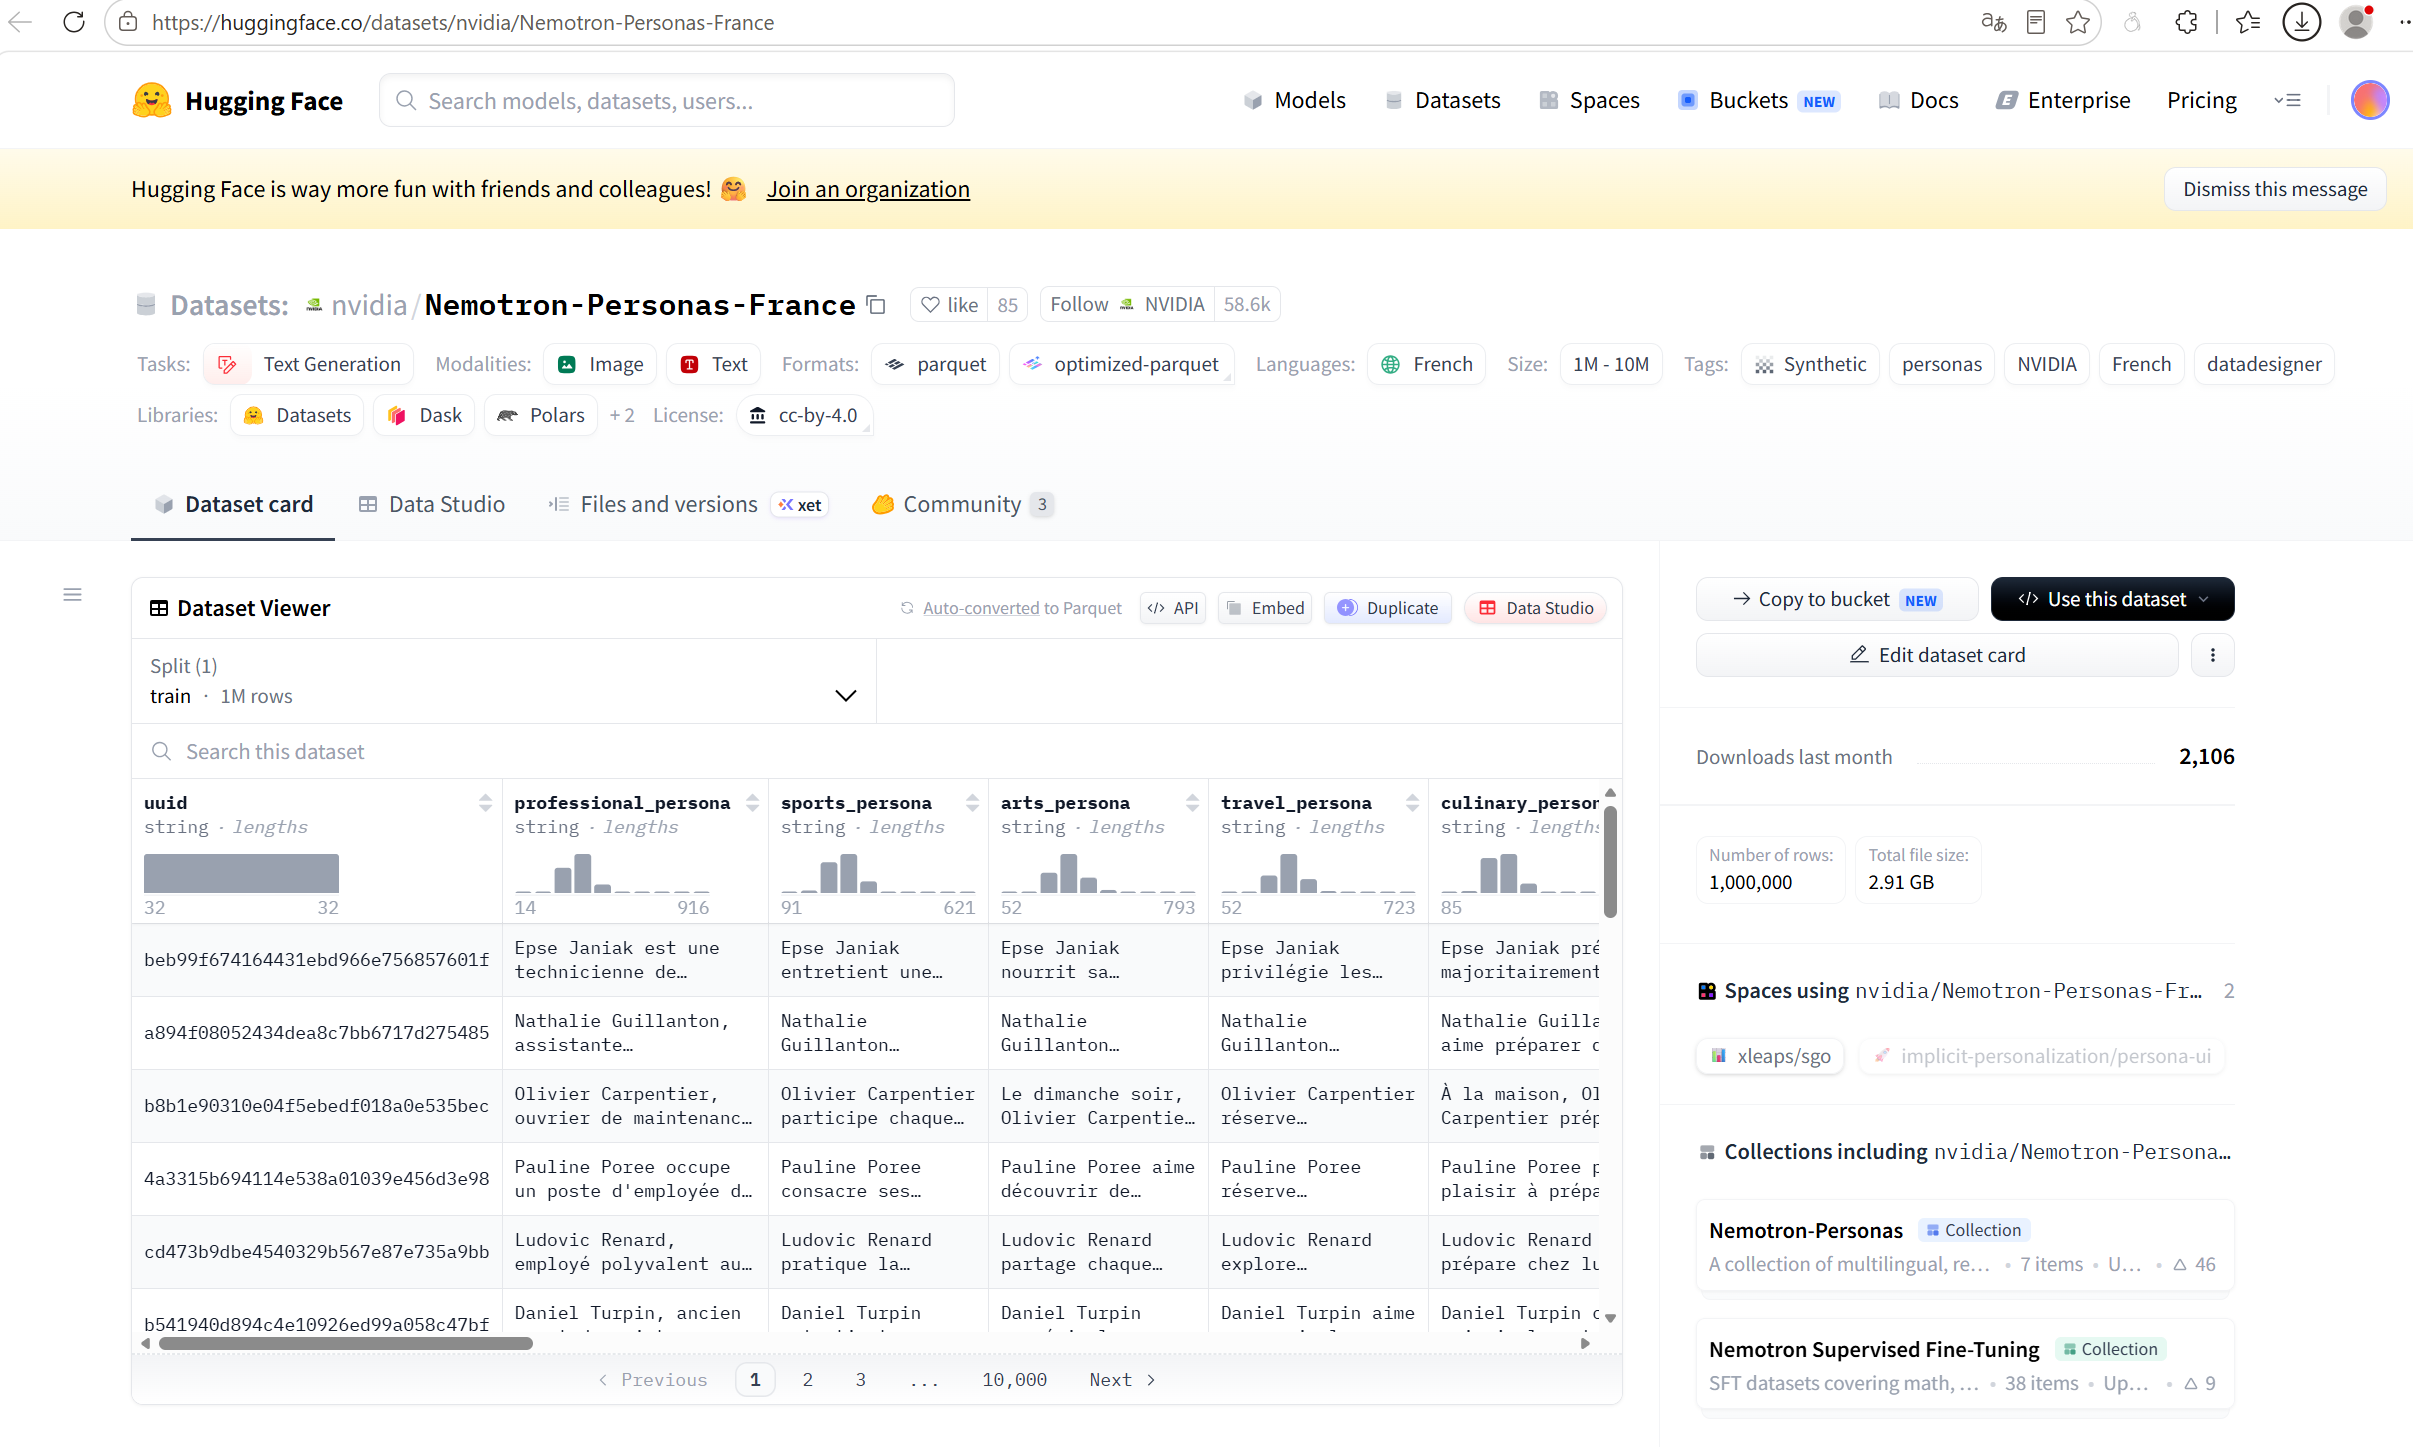
\includegraphics[width=0.92\textwidth]{figures/huggingface_source.png}
  \caption{\dataset{} 的数据来源页面。项目最初由该合成法国人物画像数据集出发，将其从一般 persona 数据重新组织为模拟社会调查的候选受访者库。}
  \label{fig:data_source}
\end{figure}

这些数据并不是真实个人信息，而是合成 persona。因此，我们将其定位为“模拟调查的输入材料”，而不把它视为真实法国人口样本。也正因为如此，后续必须引入真实民调作为宏观参照。

\subsection{LLM 社会调查模拟系统}
在明确数据来源后，项目的核心问题变成：如何把静态人物画像转化为可分析的模拟调查数据？整个系统流程可以概括为：人物画像数据库 $\rightarrow$ 抽样策略 $\rightarrow$ Prompt 构建 $\rightarrow$ LLM 调用 $\rightarrow$ JSON 解析 $\rightarrow$ 质量审计 $\rightarrow$ 主数据集构建。模型输出被要求包含三个核心字段：0--10 的支持度评分 \score{}、三分类立场标签 \stance{}，以及一句解释理由 reason。

\begin{figure}[H]
  \centering
  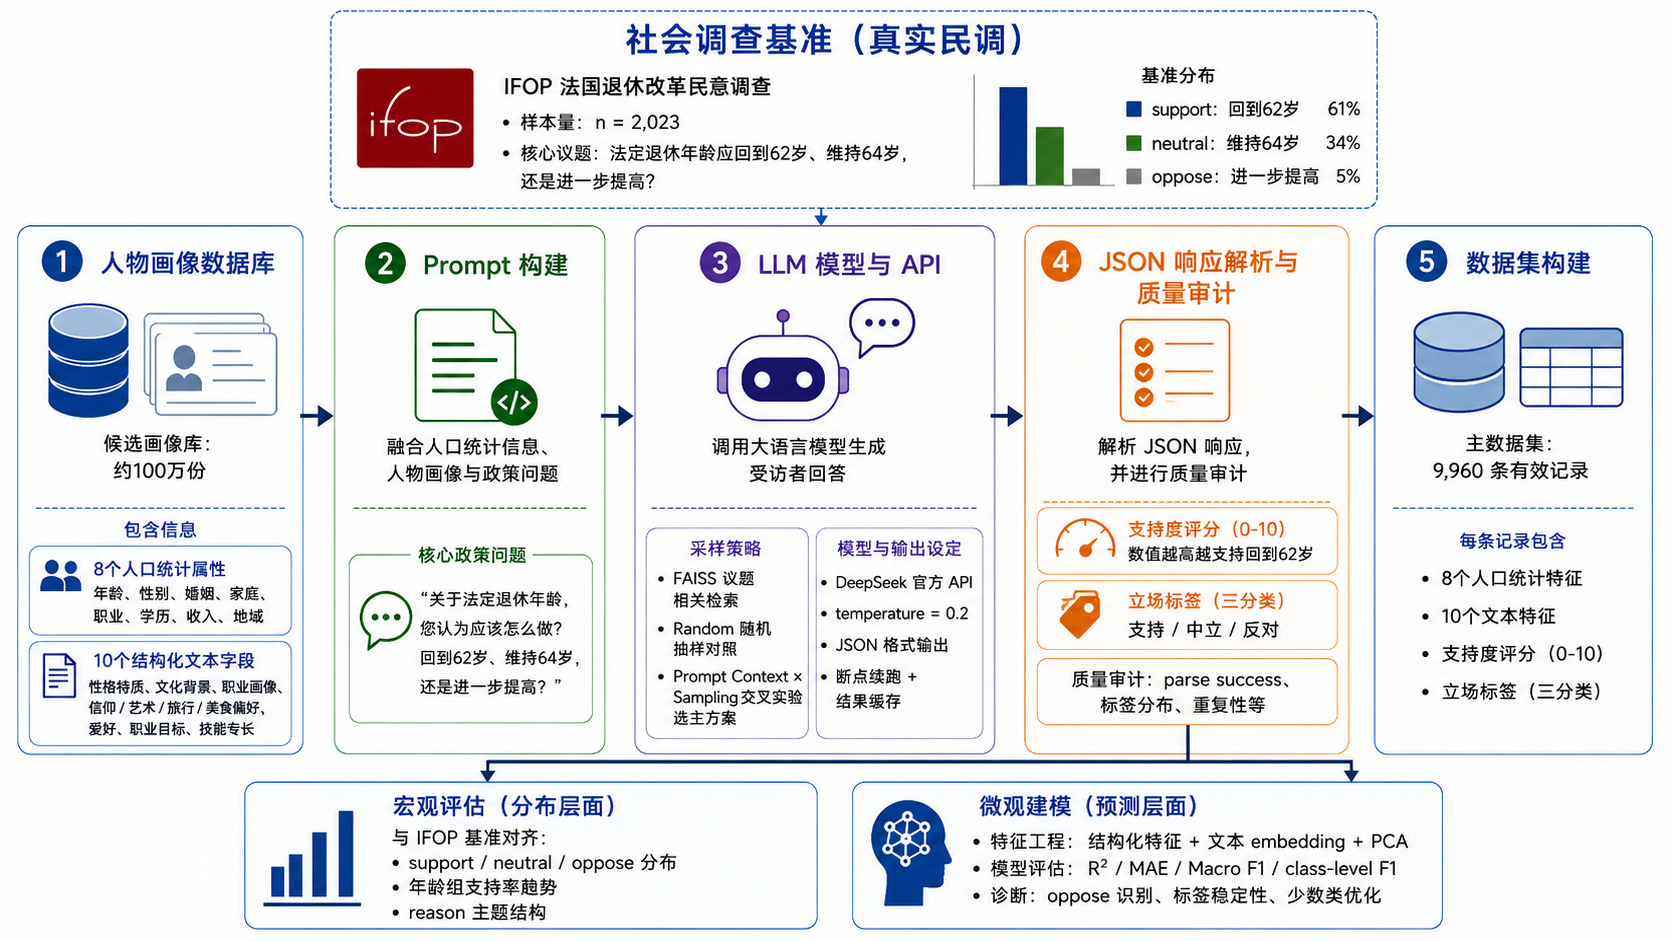
\includegraphics[width=0.98\textwidth]{figures/system_architecture.png}
  \caption{LLM 社会调查模拟系统架构。系统以真实民调作为宏观基准，从人物画像数据库中抽样并构造 Prompt，经 LLM 生成受访者回答，再通过 JSON 解析和质量审计形成主数据集，最后进入宏观评估和微观建模两个分析层面。}
  \label{fig:pipeline}
\end{figure}

最终主数据集包含 9,960 条有效记录。后续所有探索性分析和建模实验均基于这一冻结版本数据进行，不再重新调用 API。

\subsection{真实民调基准与输出标签}
为了评价模拟结果是否具有现实参照意义，我们选取 \ifop{} 关于法国退休改革的民调作为 Ground Truth \cite{ifop2023pension}。该民调关注的问题是：法定退休年龄应该回到 62 岁、维持 64 岁，还是进一步提高？我们将三类回答映射为：

\begin{itemize}
  \item \textit{support}：支持回到 62 岁；
  \item \textit{neutral}：维持 64 岁；
  \item \textit{oppose}：进一步提高。
\end{itemize}

真实基准中的总体分布约为 61\% support、34\% neutral、5\% oppose。这个分布为后续抽样和宏观评估提供了参照。

\subsection{前端系统与交互式展示}
除了离线分析脚本，我们还实现了一个 Streamlit 前端系统，用于展示项目从人物画像检索到 LLM 模拟回答的交互过程。前端入口为 \texttt{app.py}，主要功能包括：加载本地人物画像与向量索引、根据查询检索相似 persona、构造政策问题 Prompt、展示模型返回的支持度评分、立场标签和 reason，并将模拟结果以图表形式呈现。该系统并不是最终建模的必要步骤，但它帮助我们把“LLM 社会调查模拟”从静态数据表转化为可以交互检查的工作流，也方便在汇报中展示项目实际实现。

\begin{figure}[H]
  \centering
  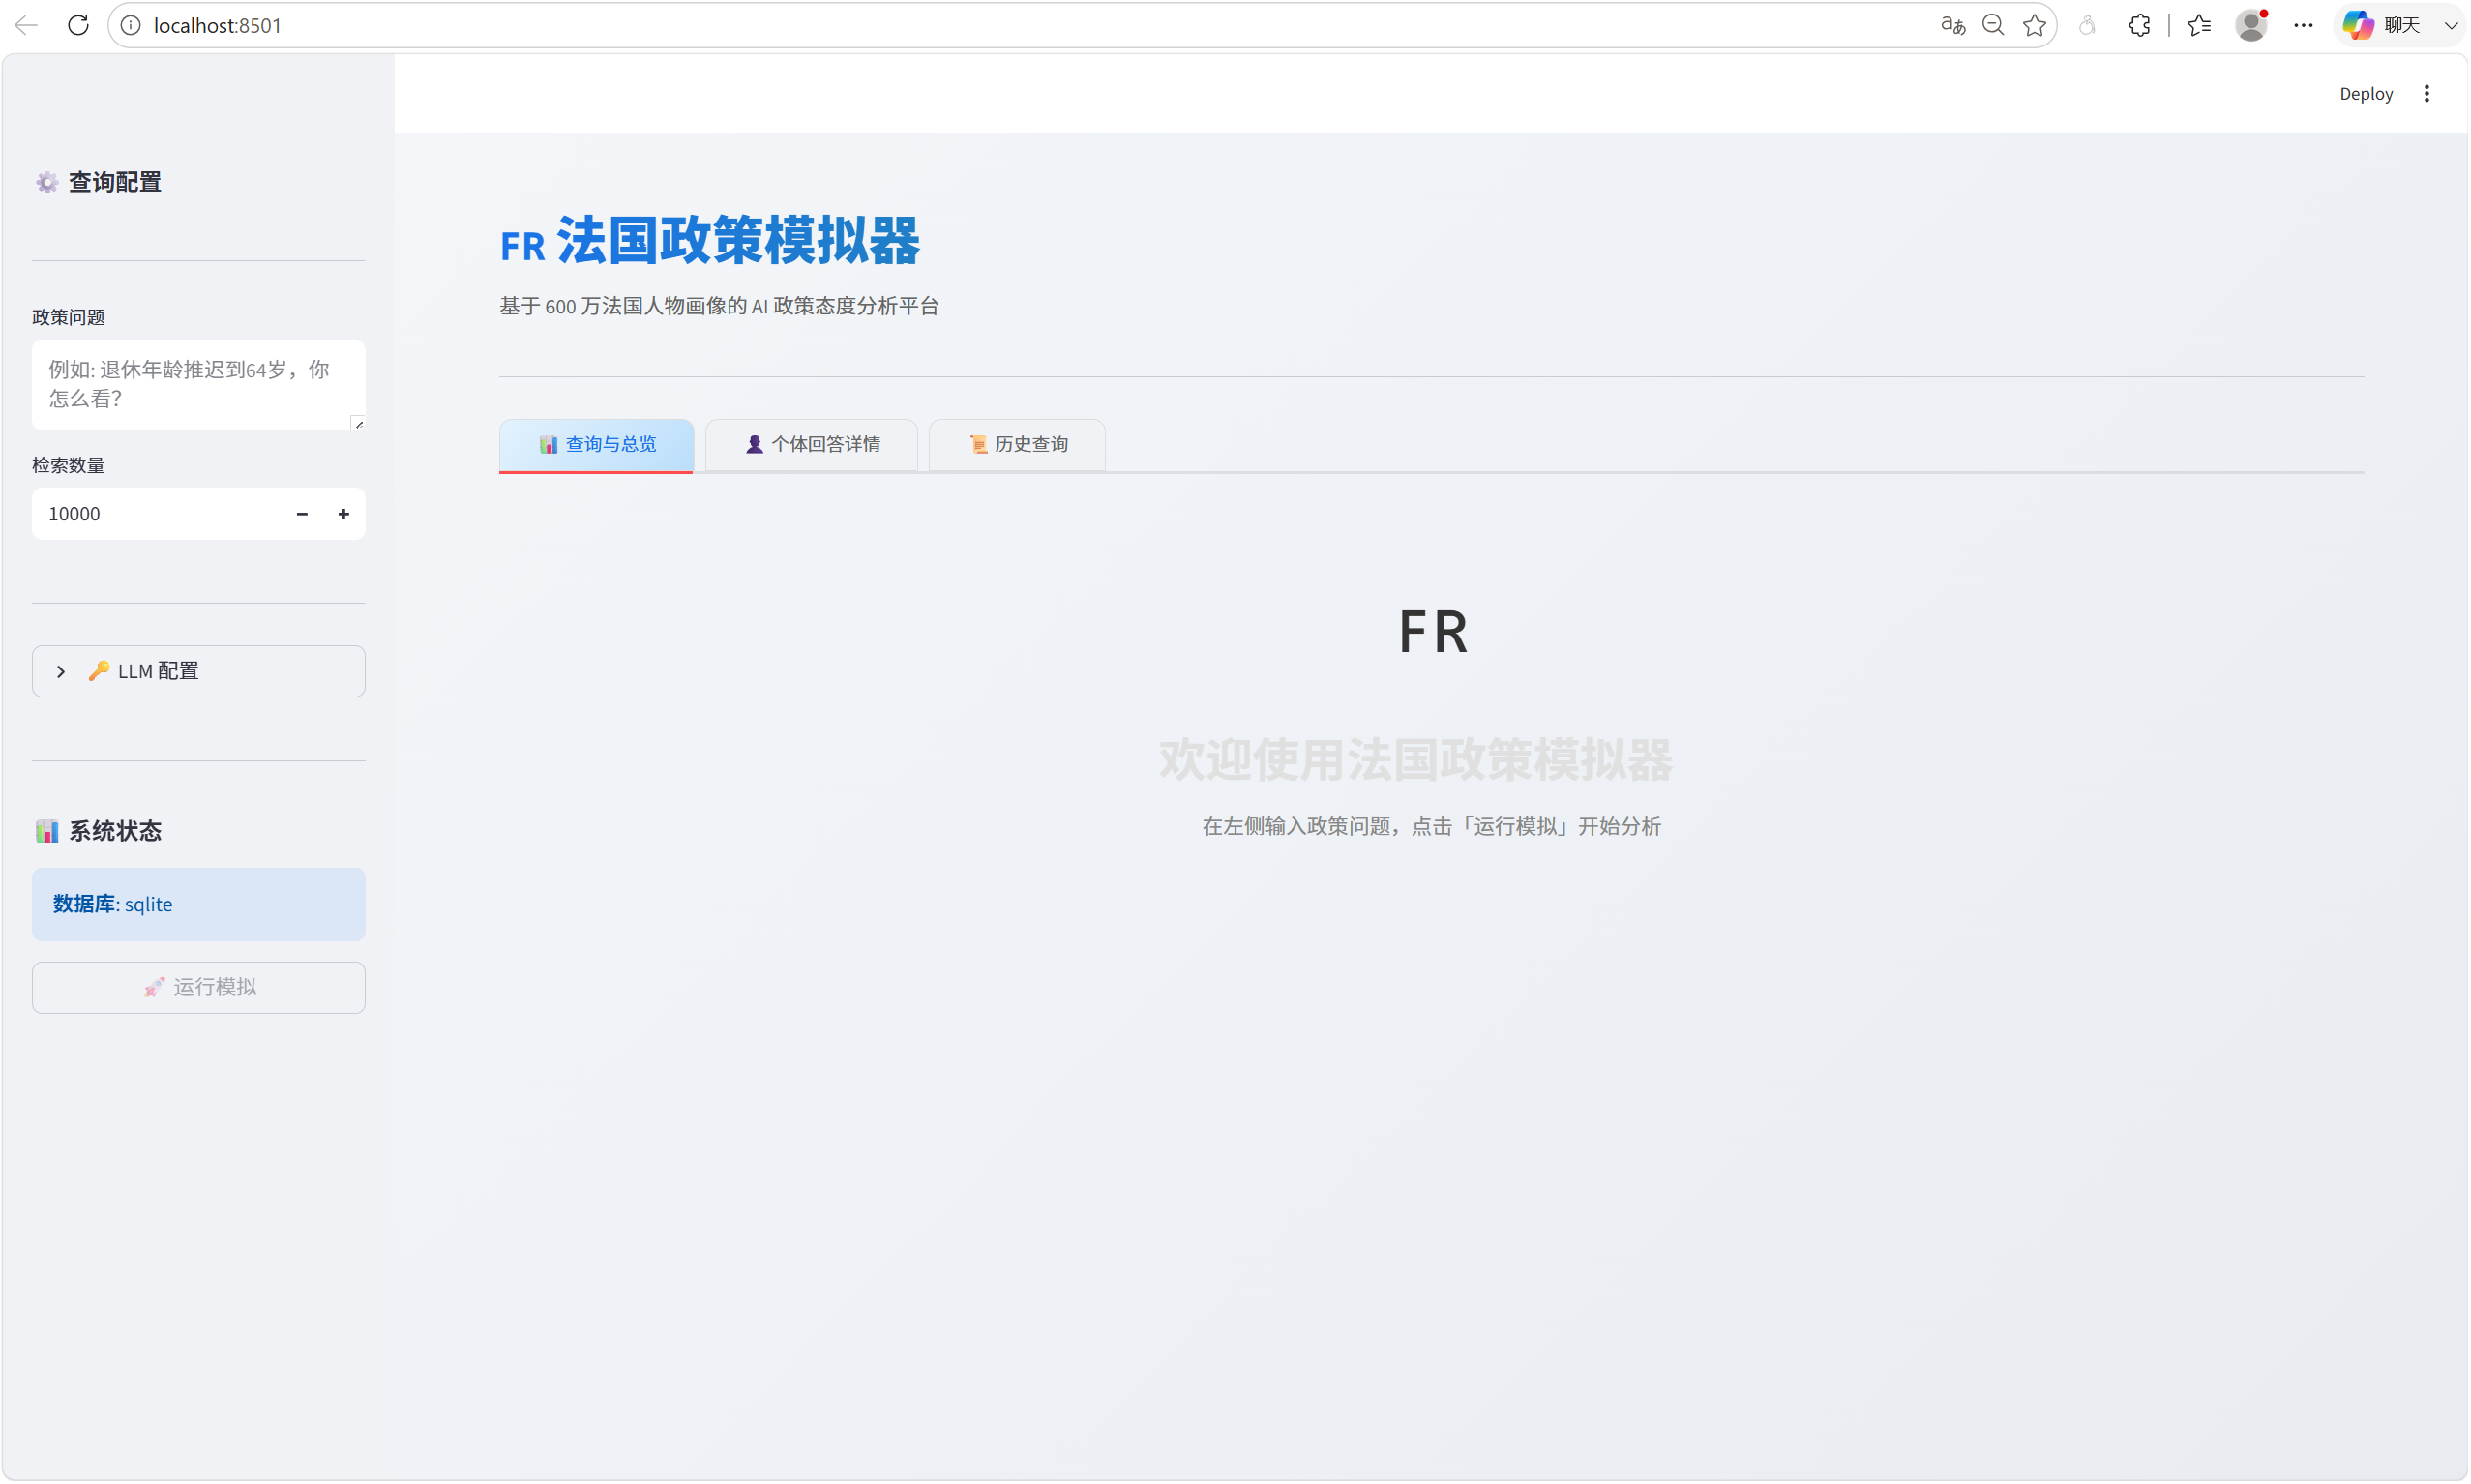
\includegraphics[width=0.92\textwidth]{figures/frontend_screenshot.png}
  \caption{前端系统运行界面。系统以 Streamlit 实现，左侧提供政策问题、检索数量和 LLM 参数配置，主界面用于展示查询总览、个体回答详情与历史查询结果。它不是单纯展示页面，而是项目数据生成流程的可交互入口。}
  \label{fig:frontend}
\end{figure}

\section{Prompt $\times$ Sampling：主数据生成方案的探索}
在正式生成主数据之前，我们首先进行了抽样和 Prompt Context 的交叉实验。这个阶段不是技术细节的附属部分，而是本项目评估统计真实性的第一步：如果样本选择和提问信息本身已经强烈偏置，那么后续 EDA 和建模结果都会建立在不可靠的数据基础上。

我们将这个问题拆成两个维度。第一是 Sampling，即“问谁”。纯随机抽样最简单，也最能避免人为筛选，但它不一定能保留与真实民调相关的人口结构；FAISS 相似度检索可以根据真实调查样本附近的人物画像进行选取，使样本更接近目标分布，但也可能带来样本偏置和画像相似度过高的问题。第二是 Prompt Context，即“告诉模型多少受访者信息”。更完整的 persona 文本可能帮助模型理解个体背景，但也可能引入无关信息、刻板联想或过强的叙事暗示。

因此，我们把不同抽样策略与不同 Prompt Context 交叉组合，记录 API 成功率、JSON 解析成功率、立场分布、support 与 \ifop{} 基准的偏差、以及理由文本的可解释性。这个实验的目的不是寻找一个绝对最优 Prompt，而是在主数据生成之前排除明显不可用的方案，并选择一个在宏观拟合、解析稳定性和信息完整性之间相对平衡的组合。交叉实验的主要结果汇总于表~\ref{tab:prompt_sampling}。

\begin{table}[H]
\centering
\caption{Prompt $\times$ Sampling 交叉实验主要结果。每组 2,000 条样本；IFOP 基准为 support 61\%、neutral 34\%、oppose 5\%。}
\label{tab:prompt_sampling}
\begin{tabular}{llrrrr}
\toprule
Sampling & Prompt Context & Support & Neutral & Oppose & 分布 MAE \\
\midrule
FAISS & P2 完整画像 & 64.75\% & 32.15\% & 3.10\% & \textbf{2.50} \\
Random & P2 完整画像 & 68.25\% & 29.70\% & 2.05\% & 4.83 \\
Random & P3 压缩全字段 & 70.55\% & 27.80\% & 1.65\% & 6.37 \\
FAISS & P3 压缩全字段 & 71.65\% & 27.35\% & 1.00\% & 7.10 \\
Random & P1 职业信息 & 73.85\% & 23.70\% & 2.45\% & 8.57 \\
FAISS & P1 职业信息 & 77.95\% & 20.20\% & 1.85\% & 11.30 \\
Random & P0 人口统计 & 78.45\% & 15.80\% & 5.75\% & 12.13 \\
FAISS & P0 人口统计 & 82.05\% & 14.25\% & 3.70\% & 14.03 \\
\bottomrule
\end{tabular}
\end{table}

最终用于主数据生成的方案是 FAISS 抽样加完整文本画像。一次 10,000 条生成实验中，API 成功率约为 99.7\%，JSON 解析成功率约为 90.0\%，模拟得到的 support 占比约为 66.8\%，与 \ifop{} 基准的 support 比例相差约 5.8 个百分点。该结果并不完美，但它通过了主数据构建的最低门槛：既能形成足够规模的结构化记录，也能在宏观分布上接近真实调查，并保留可供后续分析的文本理由。

\section{主数据探索性分析}
图 \ref{fig:eda} 展示了主数据的几个基本特征。首先，模拟数据的立场分布与 \ifop{} 基准在大方向上相似：support 是多数类，neutral 次之，oppose 最少。其次，年龄与支持度之间存在明显方向性关系，年龄越高，支持回到 62 岁的比例越高。第三，\score{} 分布集中在中高分区间，说明模型倾向于生成较多支持或温和支持态度。

\begin{figure*}[t]
  \centering
  \begin{subfigure}{0.32\textwidth}
    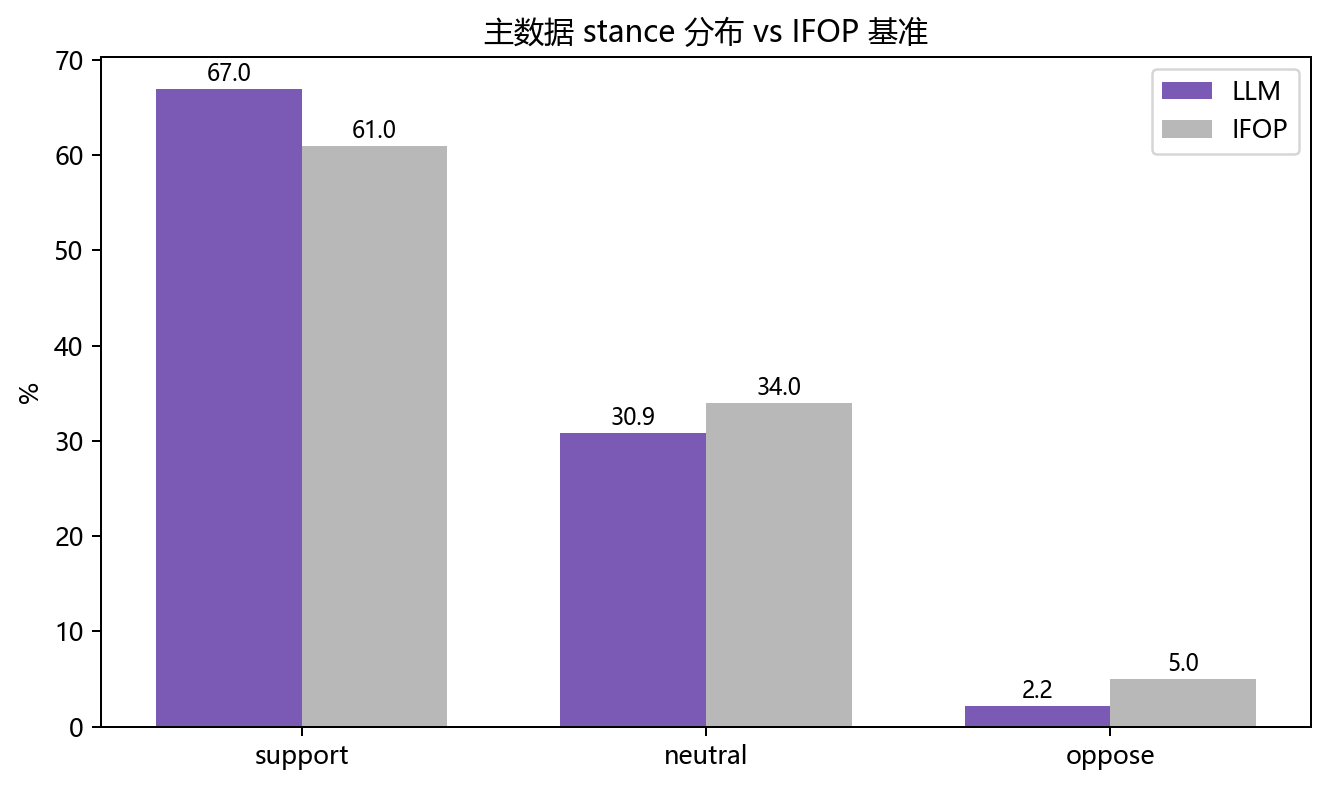
\includegraphics[width=\linewidth]{figures/stance_vs_ifop.png}
    \caption{模拟立场与 IFOP 基准对比}
  \end{subfigure}
  \hfill
  \begin{subfigure}{0.32\textwidth}
    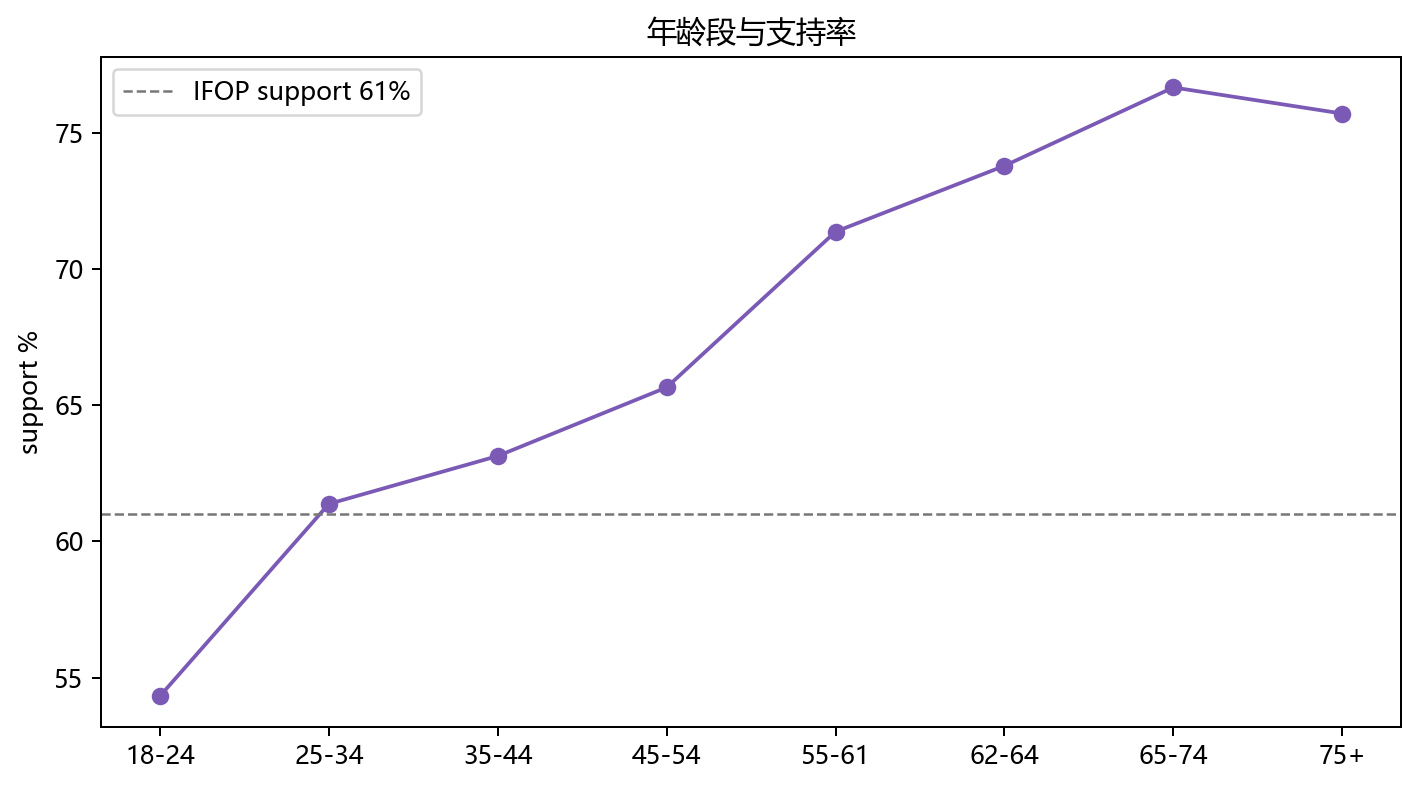
\includegraphics[width=\linewidth]{figures/age_group_support.png}
    \caption{不同年龄组支持率}
  \end{subfigure}
  \hfill
  \begin{subfigure}{0.32\textwidth}
    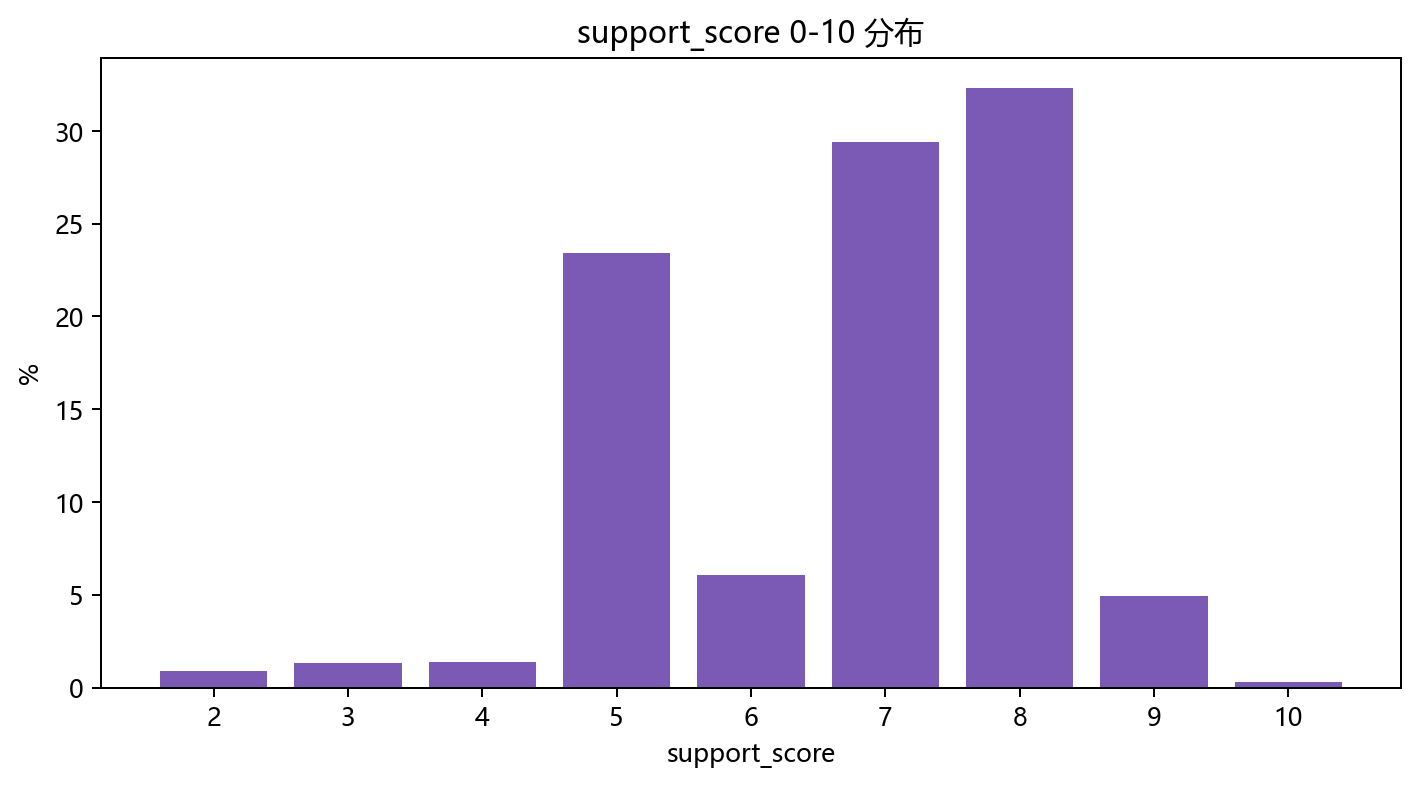
\includegraphics[width=\linewidth]{figures/score_distribution.png}
    \caption{支持度评分分布}
  \end{subfigure}
  \caption{主数据探索性分析。模拟数据中存在可解释的群体结构信号，尤其是年龄与支持度之间的关系。}
  \label{fig:eda}
\end{figure*}

这些现象说明，主数据不是完全随机噪声，其中确实包含一定社会结构信号。

此外，我们进一步检查了 LLM 生成的理由文本。图~\ref{fig:reason_wordclouds} 展示了三类立场理由的关键词词云。可以看到，年龄、工作、经济、家庭等主题在不同立场中反复出现，表明 LLM 并非随机给出理由，而是调用了可辨识的社会语义线索。但同时，三类关键词之间存在明显重叠——neutral 和 oppose 都倾向使用"稳定""谨慎""务实"等词汇——这暗示少数类的语义边界并不清晰，后续建模可能面临标签区分困难。

同时，分数集中和少数类稀缺也提示我们：后续建模可能会遇到解释力有限和类别不平衡问题。

\begin{figure}[H]
  \centering
  
\includegraphics[width=0.96\textwidth]{figures/reason_wordclouds_panel.png}
  \caption{三类立场理由关键词词云。从左到右依次为 support、neutral 和 oppose。三类词云存在明显关键词重叠，尤其是 neutral 和 oppose 共享较多"稳定""谨慎"等词汇，说明少数类理由语义并非完全独立。}
  \label{fig:reason_wordclouds}
\end{figure}

\section{特征工程、建模与诊断}
在主数据标签 $y$ 固定之后，后续建模不再改变 LLM 生成的态度结果，而是比较不同人物画像表示方式能否解释这些结果。项目可用的输入信息包含两大类：一部分是人口统计和社会结构变量，另一部分是职业、生活方式、兴趣、文化背景等文本画像。因此，特征工程也自然分成两条线：先从最可解释的结构化社会变量开始，再尝试引入高维文本语义。

\subsection{第一轮：结构化特征与多类模型}
第一轮实验固定标签 $y$，只比较不同输入特征 $X$ 和不同模型复杂度。实验设计同时检验两个维度：特征编码能否捕获更多社会结构信息，以及模型复杂度能否从同组特征中提取更强的预测信号。我们构造了四组结构化特征：

\begin{itemize}
  \item \textbf{A0 Label}：最低复杂度基线，使用标签或有序编码；
  \item \textbf{A1 One-hot}：展开类别变量，避免人为引入顺序关系；
  \item \textbf{A2 Age+}：加入年龄段、临近退休等与政策相关的年龄机制；
  \item \textbf{A3 Social}：合并职业、学历等社会分组，降低类别噪声。
\end{itemize}

模型方面，我们从简单到复杂依次使用线性模型、Ridge、随机森林、XGBoost 和 LightGBM。线性模型和 Ridge 检验退休态度是否能由社会人口变量的可加性效应近似描述；随机森林捕捉非线性和特征交互；XGBoost 和 LightGBM 则进一步提高模型容量，检验更复杂的 Boosting 算法能否从有限的低维特征中榨取额外信息。将上述 4 组特征与 5 类模型完整交叉，共得到 20 组实验，统一使用 5 折交叉验证调参与独立测试集评估。

\begin{figure}[htbp]
  \centering
  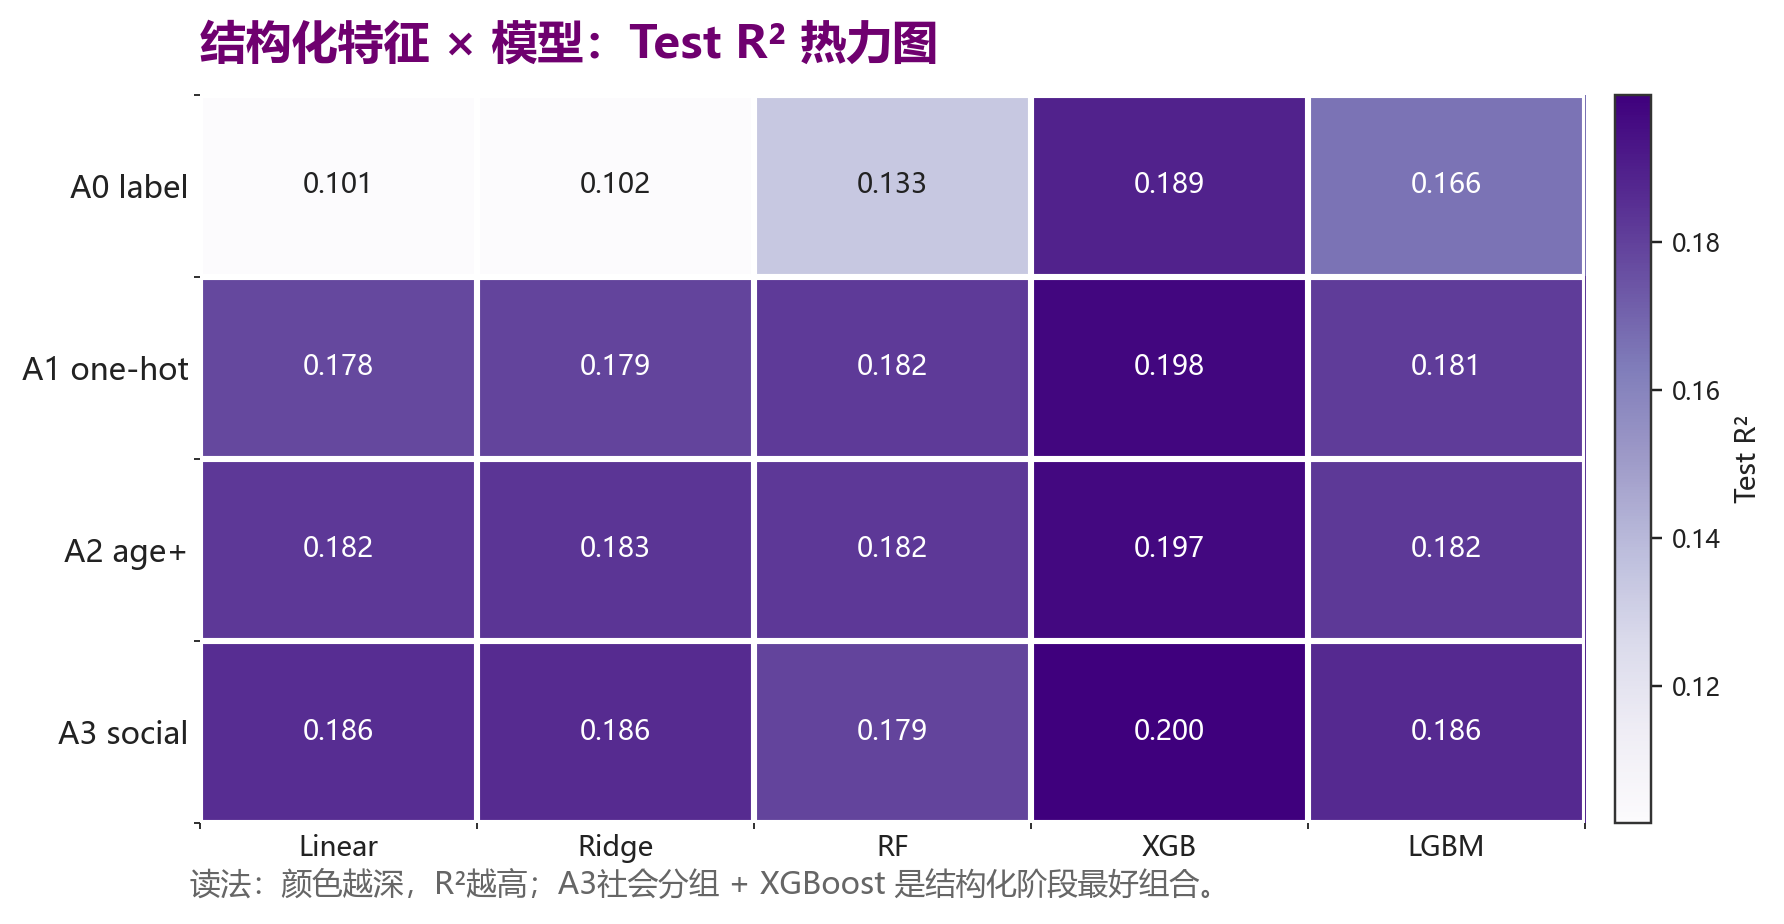
\includegraphics[width=0.85\textwidth]{figures/structured_r2_heatmap.png}
  \caption{第一轮建模结果：结构化特征与模型组合的 Test $R^2$。XGBoost 表现最稳定，但四种特征方案之间差异很小，最佳 $R^2$ 约为 0.200。}
  \label{fig:modeling1}
\end{figure}

结果如图 \ref{fig:modeling1} 所示。从热力图中可以读出三个层次的信息。第一，模型复杂度确实带来了提升：线性模型和 Ridge 在四种特征方案下的 $R^2$ 均不超过 0.12，随机森林提升到 0.16--0.18 区间，而 XGBoost 达到约 0.200。效果提升主要发生在从线性模型到 Boosting 的跨越，而非从随机森林到 Boosting 的微调。第二，在同一模型族内部，特征方案的差异很小：XGBoost 下 A1、A2、A3 的 $R^2$ 差距不到 0.01，说明继续调整结构化编码的边际收益极低。第三，表现最好的是 A3+XGBoost 组合，但其 $R^2$ 也只有约 0.200，意味着结构化变量对支持度评分的解释力上限大约在五分之一方差左右。这说明在结构化社会变量空间内，依靠增加编码精度或微调社会分组，已经很难获得实质性突破。下一轮实验的方向因此转向人物画像中的文本信息。

\subsection{第二轮：文本画像特征}
由于结构化特征已进入平台期，我们进一步检验 persona 文本是否能提供结构化变量之外的额外信息。每个 persona 的文本画像（职业描述、生活方式、兴趣爱好、文化背景等）通过 all-MiniLM-L6-v2 模型转换为 384 维 SBERT 嵌入，再根据实验方案决定是否进行 PCA 降维。模型端仅保留线性模型和 XGBoost 作为代表，维持与第一轮相同的数据划分、交叉验证和评估标准。

实验共设计五组方案，各自对应不同的假设：
\begin{itemize}
  \item \textbf{T0（结构化基线）}：仅使用 A3 结构化特征，作为文本方案的对照；
  \item \textbf{T1（完整文本）}：将整个 persona 文本拼接后做单条 SBERT 嵌入——假设整体语义足以编码态度线索；
  \item \textbf{T2（职业文本）}：仅使用职业相关文本——假设职业认同是养老金态度的主要文本来源；
  \item \textbf{T3（生活方式文本）}：仅使用生活方式文本——假设日常行为偏好比职业信息更能揭示价值观；
  \item \textbf{T4（分字段 PCA）}：将 persona 的多个文本字段分别嵌入，再通过 PCA 降维——假设各字段携带独立信号，降维后信号更集中。
\end{itemize}

\begin{figure}[htbp]
  \centering
  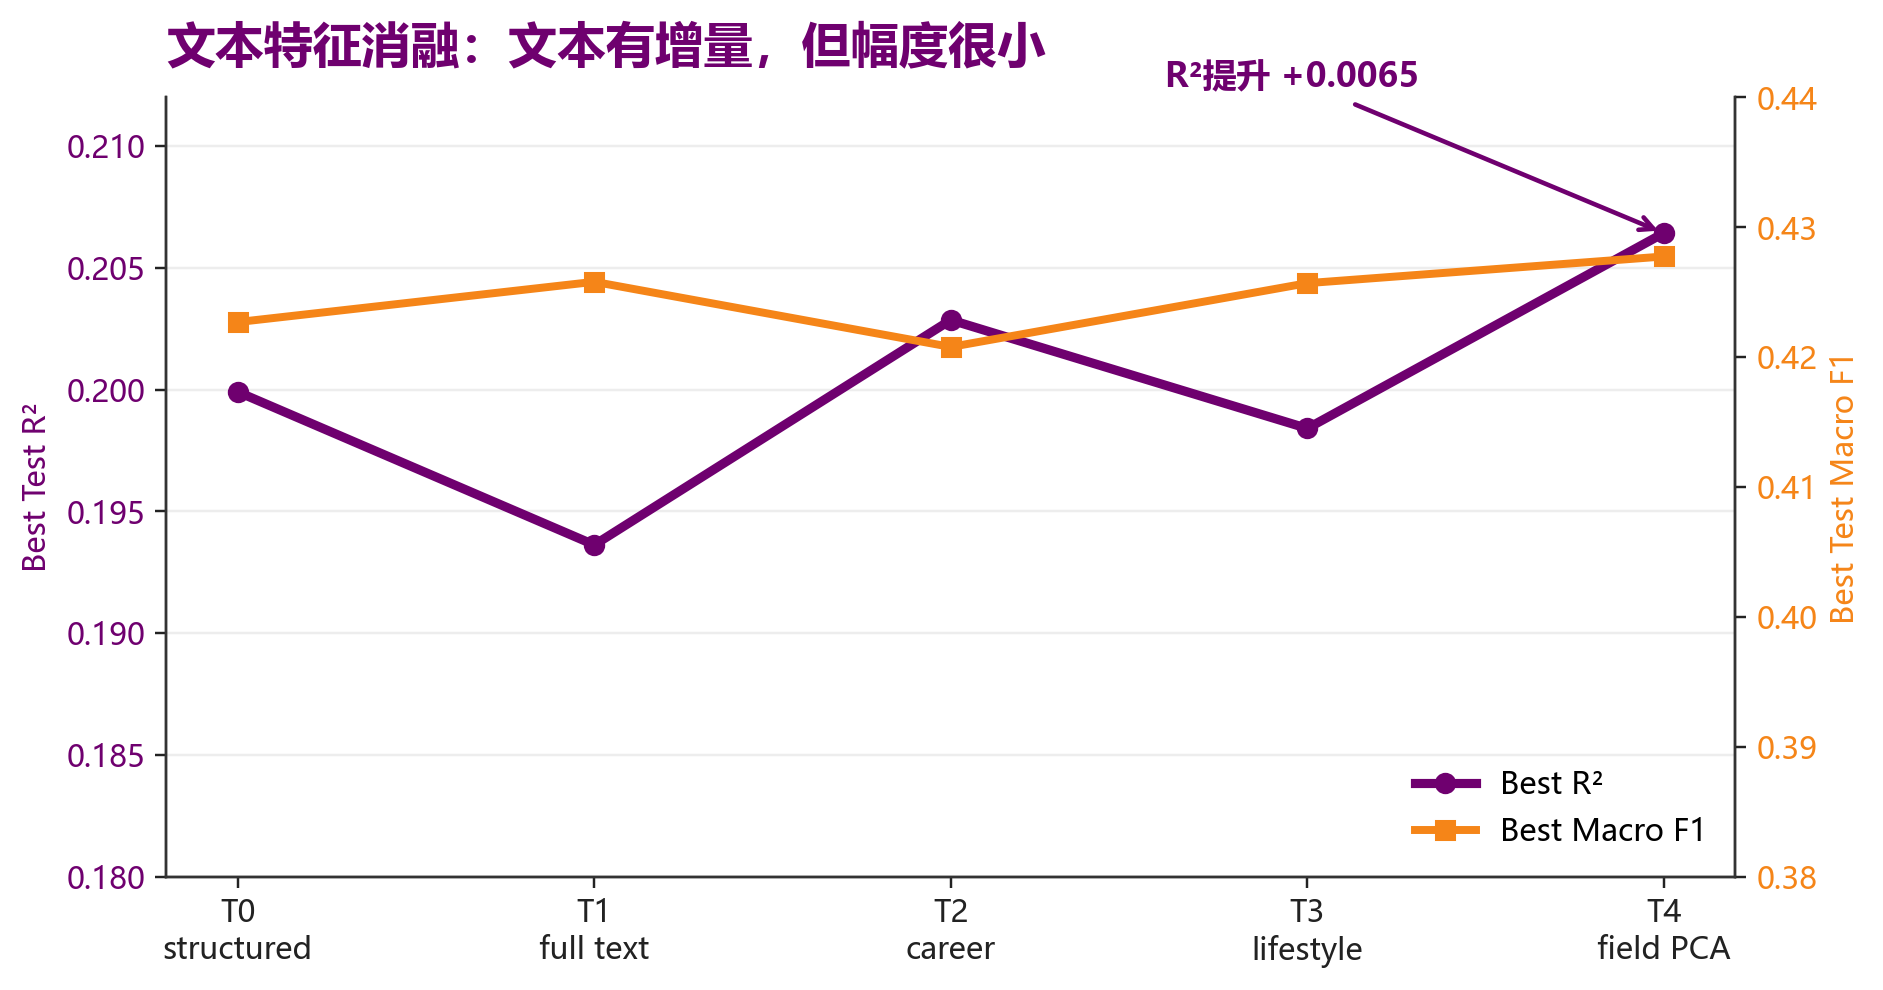
\includegraphics[width=\linewidth]{figures/text_feature_increment_lines.png}
  \caption{文本特征增量实验。T4 的效果最好，但 $R^2$ 只从约 0.200 提升到约 0.206，说明文本提供了增量信息，但没有带来质变。}
  \label{fig:textincrement}
\end{figure}

图 \ref{fig:textincrement} 从回归和分类两个指标共同评估文本方案。紫色折线（左轴）跟踪最佳测试集 $R^2$，橙色折线（右轴）跟踪 Macro F1。两组指标的变化高度一致：T1--T3 并未稳定超越结构化基线——将整段 persona 文本塞入一个 embedding（T1）、或仅依赖单一文本维度（T2、T3），效果反而可能弱于结构化特征。表现最好的 T4 将 $R^2$ 从约 0.200 略微提升至 0.206，增量仅约 0.006；Macro F1 的变化同样微小。

这一结果指向一个关键判断：文本画像虽然维度更高、内容更丰富，但其中占据主要信息量的是兴趣、生活方式和一般背景描述，未必直接关联养老金改革态度。真正更接近态度形成机制的变量——政治倾向、养老金依赖程度、工会经历、政府信任等——在 persona 数据中并不存在。

为了更直观地比较两轮实验，图 \ref{fig:dim_vs_r2} 将所有方案的特征维度与最佳测试集 $R^2$ 放在同一张散点图中。紫色点代表结构化方案 A0--A3，橙色点代表文本方案 T0--T4。横轴为编码后的特征维度（对数刻度），纵轴为最佳 $R^2$。

\begin{figure}[htbp]
  \centering
  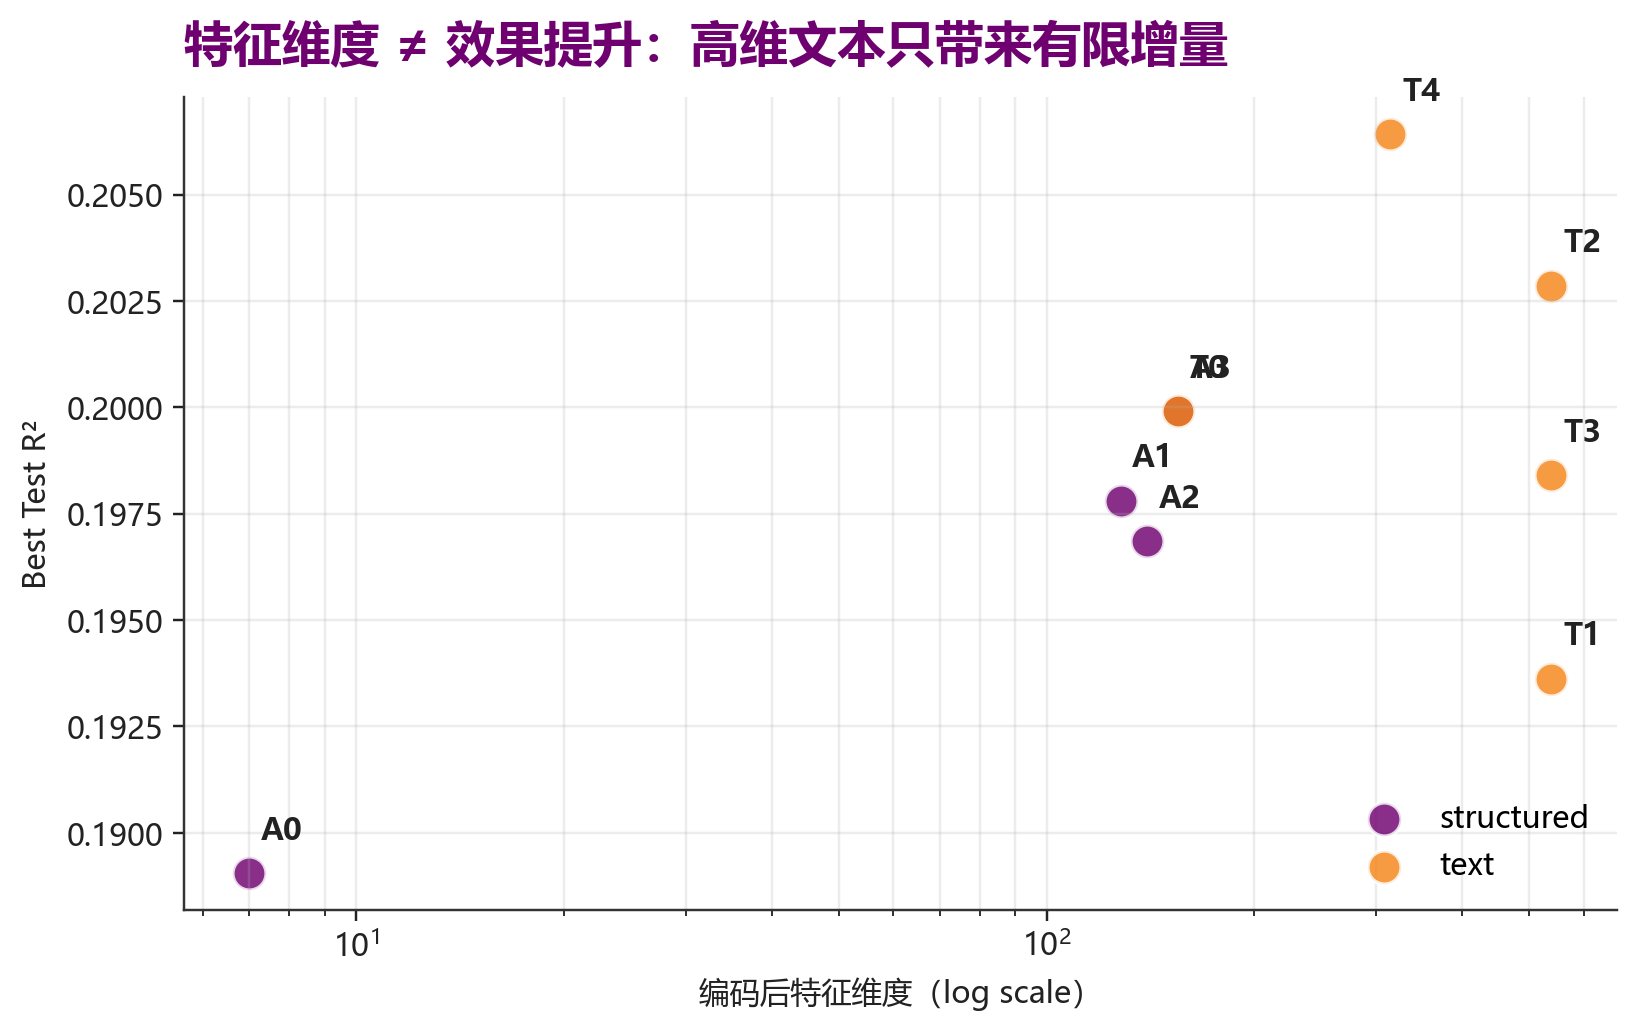
\includegraphics[width=0.85\textwidth]{figures/feature_dimension_vs_r2.png}
  \caption{两轮实验汇总：特征维度与最佳测试集 $R^2$。结构化方案（紫色）在低维区快速达到平台期；文本方案（橙色）特征维度高出 1--2 个数量级，但 $R^2$ 并未稳定超越 A3，说明特征维度增加不等于有效信息量增加。}
  \label{fig:dim_vs_r2}
\end{figure}

从图 \ref{fig:dim_vs_r2} 中可以清楚地看到，A0 维度最低、效果也最弱；A1 通过 One-hot 展开后维度与效果同步上升；但从 A1 到 A3，特征维度增加了约一倍，$R^2$ 的提升却不足 0.02——结构化方案已进入明显的平台期。文本方案 T1 和 T3 的特征维度高达 384 维，但 $R^2$ 反而低于仅有数十维的 A3；即使表现最好的 T4，相对 A3 的提升也十分微小。特征维度的增加并不等于有效信息量的增加——两个数量级的维度差距并没有换来相应的预测力提升。后续分析的重点也因此从”继续堆特征”转向”诊断模型失效的具体模式”。

\section{分类结果与少数类诊断}
除了以回归方式预测连续支持度评分 \score{}，我们还从三分类角度预测 \stance{}。分类评估之所以必要，是因为回归指标（$R^2$、MAE）可能掩盖不同立场之间的不对称表现——模型可能在多数类上拟合尚可，却完全学不到少数类的边界。由于 support 是多数类，仅看 Accuracy 容易高估模型表现，因此我们重点关注 Macro F1 以及 support、neutral、oppose 各自的 F1。

\begin{figure}[htbp]
  \centering
  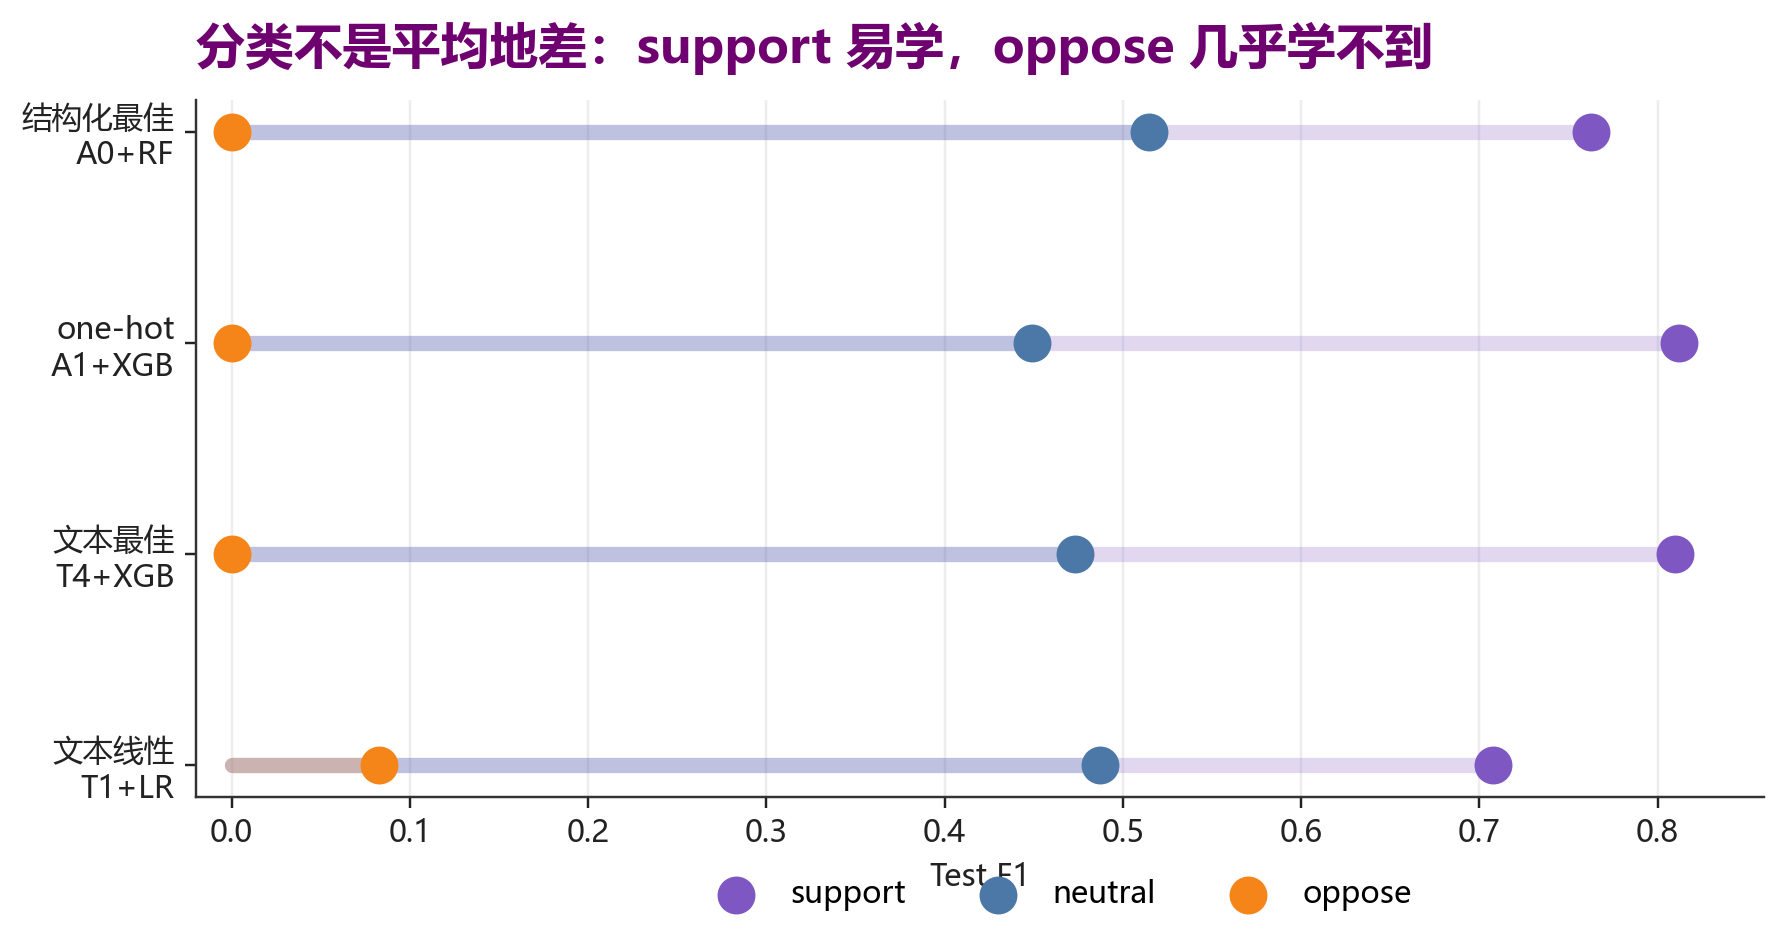
\includegraphics[width=\linewidth]{figures/class_f1_lollipop_selected_models.png}
  \caption{代表模型的类别 F1。support 较容易识别，neutral 中等，oppose 在多数直接分类模型中几乎识别不出来。}
  \label{fig:classf1}
\end{figure}

图 \ref{fig:classf1} 揭示了建模中最显著的发现之一：分类表现不是“所有类别都一样差”，而是高度不对称。左侧四个直接三分类模型中，support 的 F1 基本稳定在 0.70--0.81，neutral 集中在 0.45--0.52，而 oppose 在 XGBoost、LightGBM、随机森林中直接为 0——模型完全没有做出任何正确的 oppose 预测。只有文本线性模型（T4\_Linear）稍微突破了零值，但其 oppose F1 仍然远低于 support 和 neutral。

这种不对称有三层含义。第一，模型并非完全学不到规律——它对多数类 support 已有一定的判别力，这意味着特征空间中确实存在与态度相关的社会结构信号。第二，失败高度集中在单一类别，说明瓶颈不在模型的整体容量，而在少数类的特定性质。第三，继续以整体指标（总体 Accuracy、Macro F1）驱动模型选择，会掩盖 oppose 的识别失效；后续分析必须以 oppose 为中心展开。这使我们将诊断重点从“提升整体指标”转向“理解 oppose 为什么学不到”。

\subsection{误差结构：混淆矩阵、残差与理由语义}
为了定位 oppose 的失效模式，我们从三个角度展开诊断，分别对应预测流向、评分误差和理由语义。

\begin{figure}[htbp]
  \centering
  \begin{subfigure}{0.32\textwidth}
    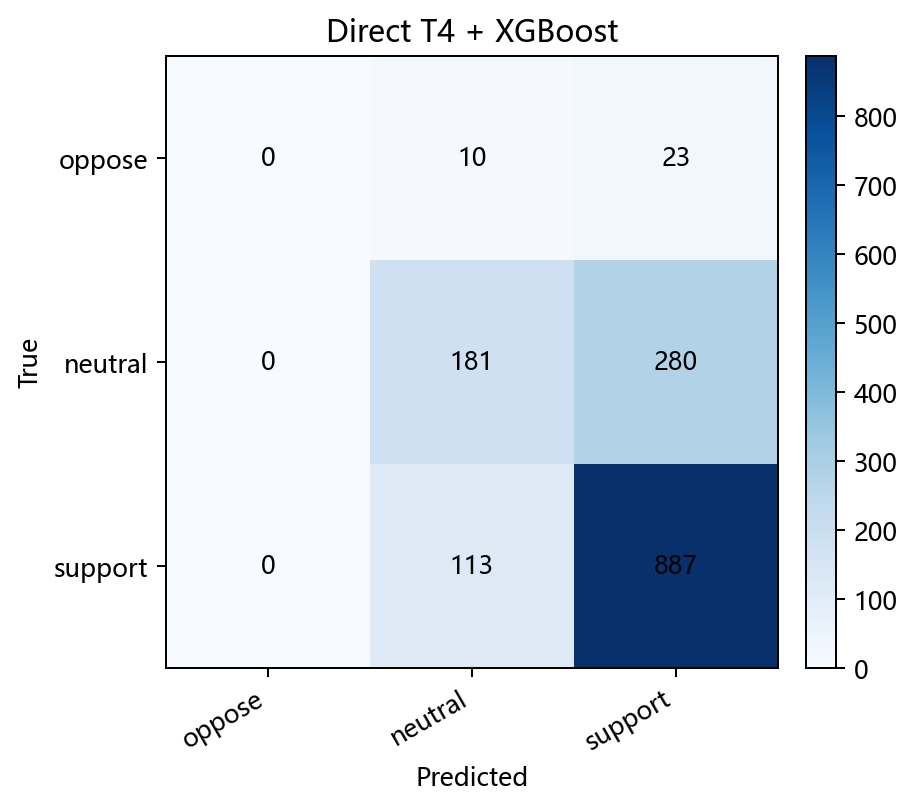
\includegraphics[width=\linewidth]{figures/direct_multiclass_confusion_matrix.png}
    \caption{直接三分类混淆矩阵}
  \end{subfigure}
  \hfill
  \begin{subfigure}{0.32\textwidth}
    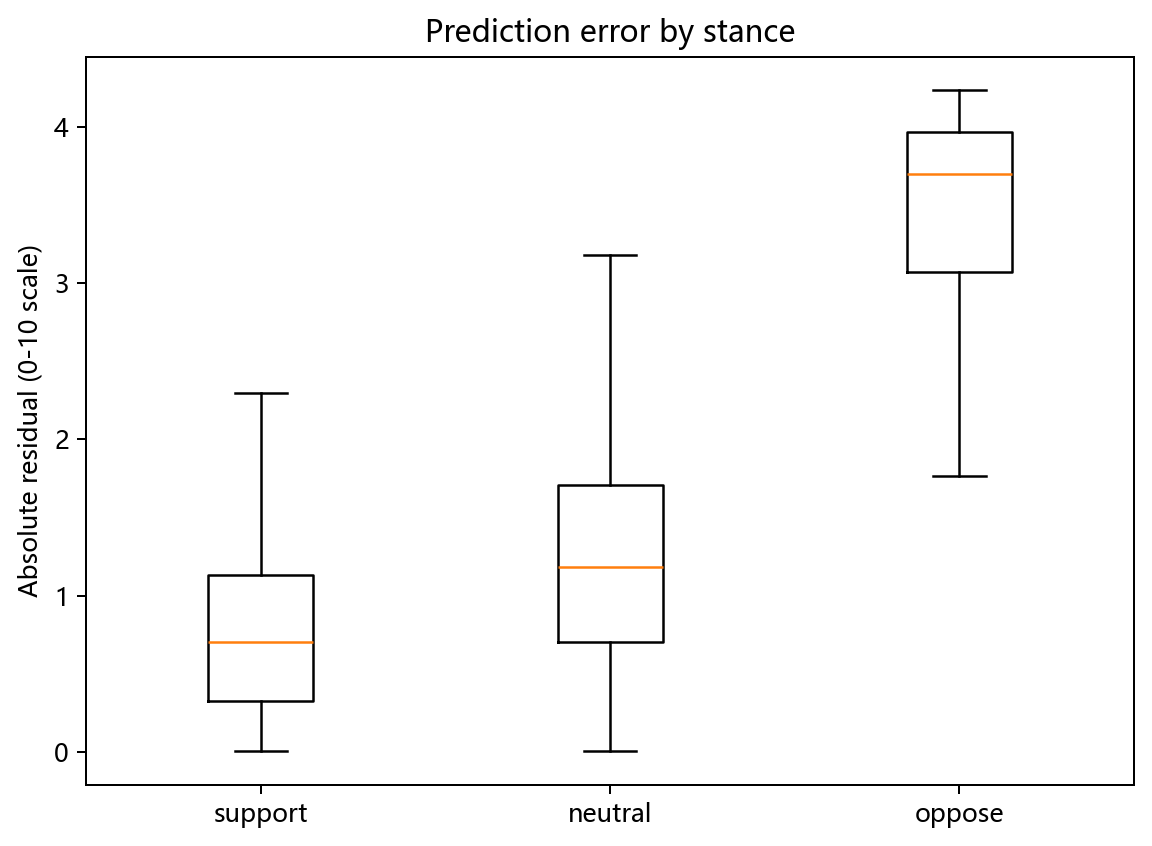
\includegraphics[width=\linewidth]{figures/absolute_residual_by_stance.png}
    \caption{不同立场的预测误差}
  \end{subfigure}
  \hfill
  \begin{subfigure}{0.32\textwidth}
    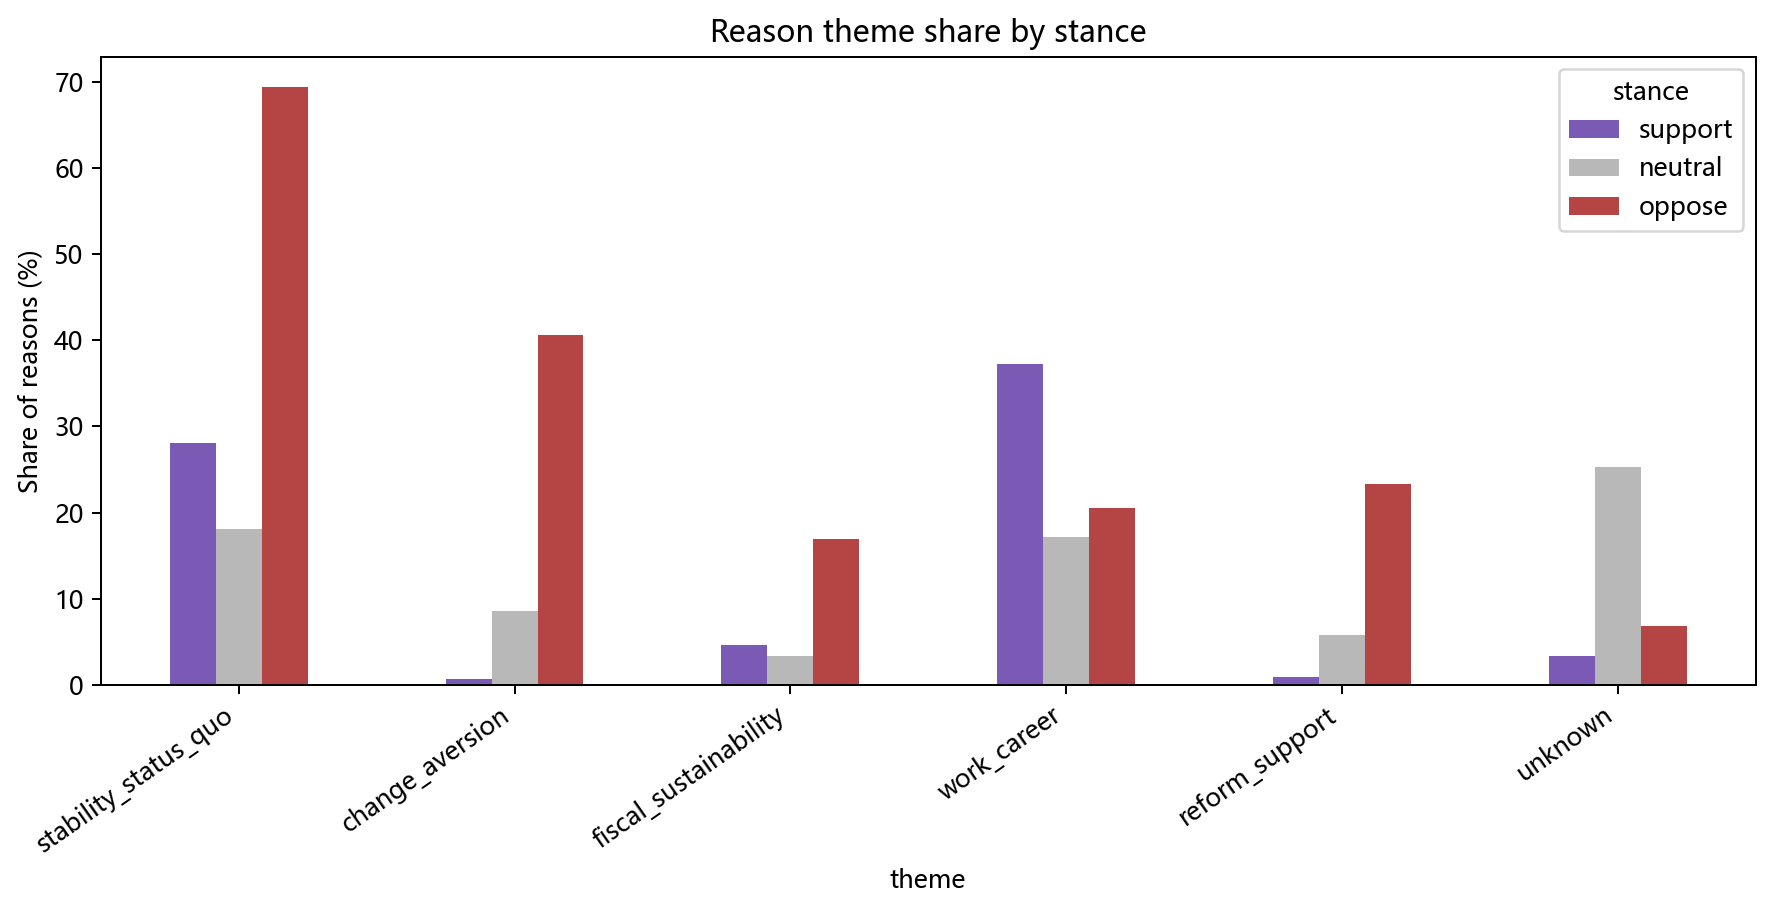
\includegraphics[width=\linewidth]{figures/reason_theme_by_stance.png}
    \caption{不同立场的 reason 主题占比}
  \end{subfigure}
  \caption{少数类诊断。oppose 不只是样本少，还存在语义来源复杂、边界与其他类别重叠的问题。三者指向同一诊断结论：oppose 在预测流向上被吸收进多数类、在评分误差上波动最大、在语义上也并非单一对立立场。}
  \label{fig:diagnosis}
\end{figure}

图 \ref{fig:diagnosis}a 的混淆矩阵直接显示了预测流向。纵轴为真实标签，横轴为预测标签。在测试集的 33 个真实 oppose 样本中，23 个被预测为 support，10 个被预测为 neutral，0 个被正确识别。换言之，模型将所有 oppose 样本“吸收”到了多数类或中间类，根本没有形成独立的 oppose 预测输出。这不是 oppose 被部分召回的问题，而是完全不可见。

图 \ref{fig:diagnosis}b 从回归残差角度验证了同一模式。箱线图展示不同 stance 下的绝对预测误差：support 的误差中位数最小、分布最紧，neutral 居中，而 oppose 的误差显著更大且更分散。模型对 support 的评分相对准确，但对 oppose 的评分系统性偏离——它倾向于给出偏高的支持度分数，从而将 oppose 样本拉向 support/neutral 区域。

图 \ref{fig:diagnosis}c 进一步从 LLM 生成的 reason 文本寻找原因。我们将 reason 关键词归纳为几类主题（年龄与退休时机、财政与制度、工作经历、改革态度与情感），并比较不同立场下的主题占比。oppose 并不呈现为 support 的“镜像”——它不是简单地反对退休改革，而是混合了财政可持续性担忧、对现行制度的谨慎维持、个人工作经历以及少量对变革的抵触情绪。这种语义上的非单一性使得 oppose 样本在文本空间中并不聚集成一个紧凑簇类，而是分散在多个主题的交界处。换言之，oppose 的内部语义变异度远大于 support，这为模型设置了一个天然的区分难度。

三种诊断——混淆矩阵的流向、残差的大小、理由主题的分布——从不同角度指向同一结论：oppose 难以识别不只是因为样本量小，还因为它本身的结构不够紧凑、与相邻类别的语义边界不够清晰。

\subsection{标签稳定性实验：如果标签本身不够稳定}
前两节从模型输出和理由语义分析了 oppose 的失效。本节进一步追问：监督学习所使用的标签本身是否足够稳定？如果 LLM 对同一 persona 在不同时刻给出不同的标签，那么即使特征完美，下游模型也不可能达到 100\% 的准确率。标签稳定性估算了 LLM 生成标签的“噪声天花板”。

我们从主数据中按原始立场分层抽取 300 个 persona（每类 100 人），使用完全相同的 Prompt 和模型参数（DeepSeek-V4-Flash, temperature=0.2）重新生成标签，每人重复两次，共 600 次调用。API 成功率 100\%，JSON 解析成功率 82\%，最终获得 492 条有效配对记录。

\begin{table}[htbp]
\centering
\caption{不同原始立场的标签稳定性}
\label{tab:stability}
\begin{tabular}{lrr}
\toprule
原始立场 & 立场一致率 & 分数 MAE（0--10） \\
\midrule
Support & 90.4\% & 0.71 \\
Neutral & 43.6\% & 1.54 \\
Oppose & 43.3\% & 2.02 \\
\bottomrule
\end{tabular}
\end{table}

表~\ref{tab:stability} 呈现了清晰的梯度：support 的立场一致率达到 90.4\%，支持度评分 MAE 仅 0.71；而 neutral 和 oppose 的一致率分别只有 43.6\% 和 43.3\%，评分 MAE 则上升到 1.54 和 2.02。换句话说，neutral 和 oppose 有一半以上的概率在第二次回答时被归入其他类别，且评分波动是 support 的 2--3 倍。

这一发现为本项目的建模效果设定了不可逾越的上限。support 的标签较为稳定，因此模型能够学到其边界；但 neutral 和 oppose 的标签本身带有约 57\% 的随机性——任何监督模型都不可能稳定地学会一个近乎随机的目标。前文观察到的 oppose F1 为 0 和 neutral F1 约 0.5，部分原因是特征和模型能力有限，但至少有同等重要的另一部分来自标签质量：LLM 自身对这两类立场的判断就处于摇摆状态。

综合误差结构诊断和标签稳定性实验，oppose 的识别困难可以归因于三重叠加因素：（1）样本稀缺——占总样本约 2--3\%；（2）内部语义不紧凑——反对理由分散在财政、稳定、工作等多个主题；（3）标签不稳定——LLM 再次生成时有超过一半的概率改变判断。三者分别对应训练信息量、语义可分性和监督信号质量，任何一个环节单独存在都难以将 oppose 学到一个可用的水平，三者叠加则使该问题在当前数据设计下几乎不可能被纯算法手段解决。

\section{优化尝试}
前述诊断表明，oppose 的识别困难同时涉及样本稀缺、语义不紧凑和标签不稳定。在改进数据和标签设计之前，我们首先尝试在现有数据约束下，通过算法手段尽可能改善 minority 识别。我们测试了四种策略：（1）\textbf{类别加权}——训练时提高 oppose 样本的损失权重；（2）\textbf{概率阈值调整}——降低预测为 oppose 的概率门槛，牺牲精确率换取召回率；（3）\textbf{回归阈值分割}——从回归预测的 support\_score 中寻找区分 oppose 的阈值；（4）\textbf{两阶段分类}——先区分 support 与非 support，再从非 support 中区分 neutral 和 oppose，通过分解任务降低类别不平衡的冲击。

\begin{figure}[htbp]
  \centering
  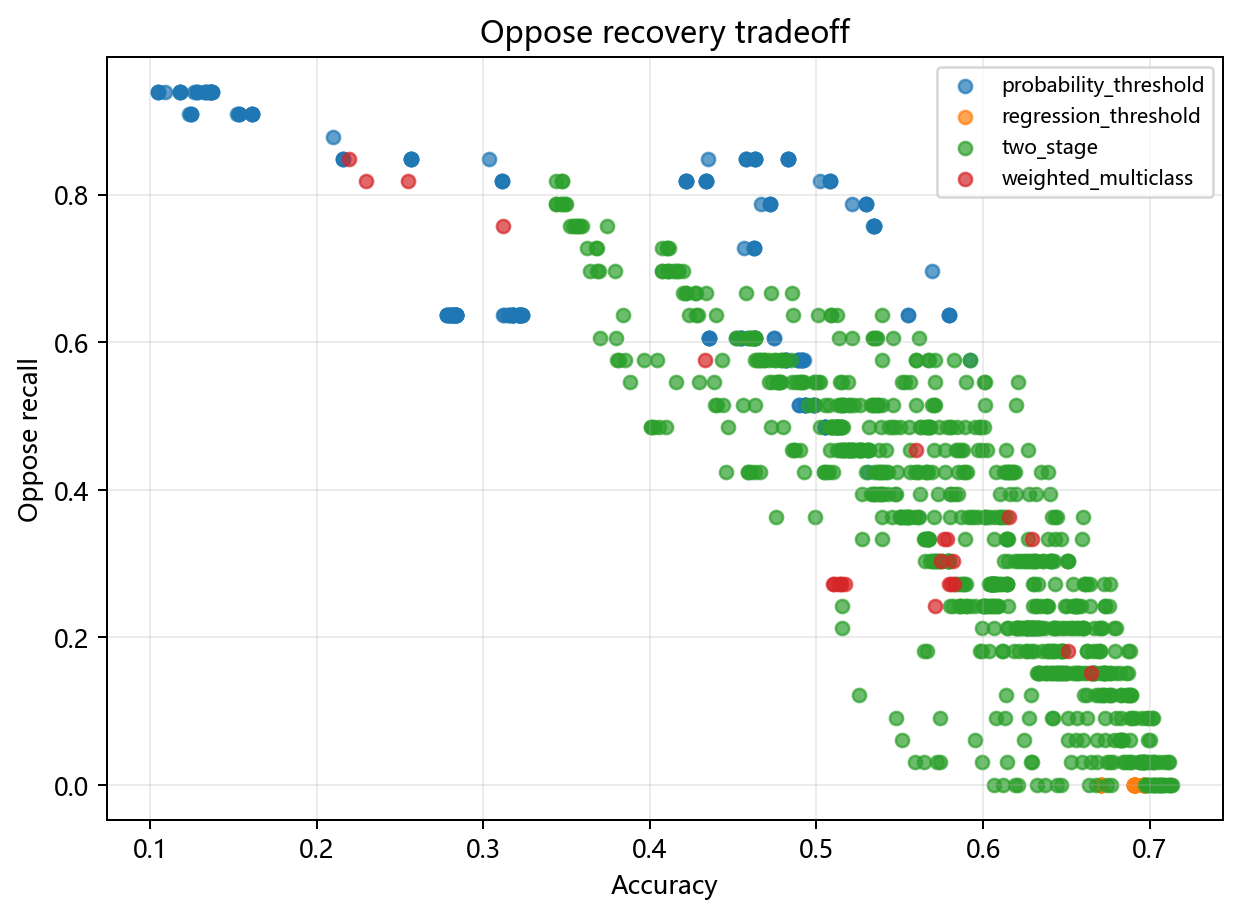
\includegraphics[width=\linewidth]{figures/oppose_recall_accuracy_tradeoff.png}
  \caption{oppose 召回率与总体准确率之间的权衡。图中不存在明显的”右上角最优点”，说明少数类优化有代价。}
  \label{fig:tradeoff}
\end{figure}

图 \ref{fig:tradeoff} 展示了不同参数配置下 oppose recall 与整体 Accuracy 的权衡关系。每个点代表一组参数组合（权重、阈值等），理想方案应位于右上角——同时保持高准确率和高 oppose 召回率。但图中并不存在这样的点：所有能将 oppose recall 推向 0.5 以上的配置，都以 Accuracy 从 71\% 跌落至 55--60\% 为代价。

\begin{table}[htbp]
\centering
\caption{代表性优化方案测试集结果}
\label{tab:optimization}
\begin{tabular}{lrrrr}
\toprule
方案 & Acc. & Macro F1 & Opp. Recall & Opp. F1 \\
\midrule
原始三分类 & 71.5\% & 42.8\% & 0.0\% & 0.0\% \\
概率阈值 & 59.2\% & 44.3\% & 57.6\% & 12.6\% \\
类别加权 & 66.5\% & 47.9\% & 15.2\% & 14.9\% \\
两阶段分类 & 67.3\% & 48.7\% & 15.2\% & 16.9\% \\
\bottomrule
\end{tabular}
\end{table}

表 \ref{tab:optimization} 汇总了代表性方案的测试集表现。概率阈值方案将 oppose 召回率从不存在的 0\% 推至 57.6\%，但这是以 Accuracy 从 71.5\% 降至 59.2\% 换来的——模型开始大量误将 neutral 甚至 support 标记为 oppose。类别加权和两阶段分类是更均衡的折衷：两阶段分类在保持 67.3\% Accuracy 的同时，将 Macro F1 从 42.8\% 提升至 48.7\%，将 oppose F1 从 0 提升至 16.9\%。但即使是最优方案，oppose F1 仍然远低于 support（0.76）和 neutral（0.53）。

综合来看，优化能够缓解少数类问题、获得非零的 oppose 识别能力，但不能根本消除。当标签本身带有约 57\% 的重测不一致率、且 oppose 的语义分布在多个主题之间时，任何纯算法优化都受到信息上限的约束。这进一步印证了前文的判断：当前系统的薄弱环节不主要在算法，而在数据生成和标签设计。

\section{讨论}
综合以上实验，本项目得到三个主要认识。

第一，LLM 模拟调查具有一定宏观可行性。模拟数据能够大致复现真实民调中 support 为多数、neutral 次之、oppose 较少的结构，也能够呈现年龄与退休改革态度之间的可解释关系。

第二，个体层面的可预测性有限。最佳回归模型的 $R^2$ 只有约 0.206，说明当前人物画像只能解释一部分支持度差异。进一步增加文本 embedding 维度并没有带来明显提升，说明“特征维度增加”不等于“有效信息增加”。

第三，建模结果有限本身具有诊断价值。oppose 难以识别并非偶然，而是由少数类样本少、语义来源复杂、标签重复生成不稳定共同造成的。这与已有研究对 LLM 合成受访者可能压平群体差异、误表征少数群体的担忧是一致的 \cite{wang2024replace,cheng2023marked}。

因此，本项目的价值不在于得到一个高分预测模型，而在于通过数据科学流程系统地识别了 LLM 模拟民调的可用部分和失效边界。

\section{局限与未来工作}
本项目仍有若干局限。首先，我们只研究了法国退休改革一个议题，结论不一定能直接推广到移民、教育、宗教等其他政策问题。其次，主数据主要来自一个 LLM 配置，未来需要比较 GPT、Claude、Qwen 等不同模型。第三，当前 persona 缺少更直接的政治态度变量，未来可以加入政党认同、政府信任、政策受益关系等特征。第四，标签稳定性实验规模仍然有限，后续可以扩大 test-retest 实验，并引入 ICC、Kappa 等更完整的信度指标。最后，如果要走向更复杂的社会模拟，还可以加入多智能体互动，观察讨论、传播和群体影响对态度分布的改变。

\section{结论}
本项目构建了一套基于人物画像和大语言模型的公共政策态度模拟流程，并以法国退休改革为案例进行了完整的数据科学分析。结果表明，LLM 可以在一定程度上生成具有社会结构信号的模拟调查数据，但其结果仍受到抽样、Prompt、人物画像信息、标签稳定性和少数类表达的限制。更准确地说，LLM 模拟调查适合作为探索性和诊断性工具，而不应被直接视为真实民调的替代品。

\section*{复现说明}
课程提交时应同时提供冻结版主数据、分析脚本和图表生成代码。本报告本身不需要重新调用 LLM API；所有分析应基于已保存的数据文件和固定随机种子完成，以保证助教能够一次运行复现主要结果。

\bibliographystyle{plain}
\bibliography{references}

\end{document}
